\documentclass[14pt]{extarticle}

\usepackage[table]{xcolor} % colored lines for tables
%\usepackage[normalem]{ulem} % strike through text
\usepackage{amsmath,mathtools,amsfonts,amsthm,amssymb,hyperref}
\usepackage{parskip,geometry,latexsym,bookmark,mathtools,float,cancel}
\usepackage{tcolorbox,bm}

\newtheorem{defn}{Definition}
\newtheorem{thm}{Theorem}
\newtheorem{claim}{Claim}
\newtheorem{lemma}{Lemma}

\newcommand{\dps}{\displaystyle}
\newcommand{\es}{\varnothing}
\newcommand{\fbl}{\underline{\hspace{1cm}}\,\,}
\newcommand{\R}{\mathbb{R}}
\newcommand{\Q}{\mathbb{Q}}
\newcommand{\Z}{\mathbb{Z}}
\newcommand{\from}{\leftarrow}
\newcommand{\true}{{\bf t}}
\newcommand{\false}{{\bf c}}
\newcommand{\bic}{\leftrightarrow}
\newcommand{\da}{\downarrow}
\newcommand{\cyda}{{\cy \(\downarrow\)}}
\newcommand{\fa}{\forall}
\newcommand{\te}{\exists}
\newcommand{\cy}{\color{cyan}}

\newcommand{\colsq}[1]{{\color{#1} $\blacksquare$}}

\newcommand{\base}[1]{{\cy #1}} % for log bases
\newcommand{\floor}[1]{{\left\lfloor#1\right\rfloor}}
\newcommand{\ceil}[1]{{\left\lceil#1\right\rceil}}
\newcommand\Ccancel[2][black]{\renewcommand\CancelColor{\color{#1}}\cancel{#2}}
\newcommand\Cbcancel[2][black]{\renewcommand\CancelColor{\color{#1}}\bcancel{#2}}

\renewcommand{\arraystretch}{1.2}

\hypersetup{colorlinks,allcolors=blue,linktoc=all}
\geometry{a4paper}
\geometry{margin=0.42in}

\title{Solutions to Chapter 9, Susanna Epp Discrete Math 5th Edition}

\author{https://github.com/spamegg1}

\begin{document}
\maketitle
\tableofcontents

\section{Exercise Set 9.1}

\subsection{Exercise 1}
Toss two coins 30 times and make a table showing the relative frequencies of 0, 1, and 2 heads. How do your 
values compare with those shown in Table 9.1.1?

\begin{proof}
\begin{center}
\arrayrulecolor{cyan}
\begin{tabular}{|c|c|c|}
\hline
{\bf\cy Event} & {\bf\cy Freq.} & {\bf\cy Rel. freq.} \\
\hline
2 heads obtained & 7 & 23.33\% \\
\hline
1 head obtained & 16 & 53.33\% \\
\hline
0 heads obtained & 7 & 23.33\% \\
\hline
\end{tabular}
\arrayrulecolor{black} % change it back!
\end{center}
\end{proof}

\subsection{Exercise 2}
In the example of tossing two quarters, what is the probability that at least one head is obtained? that coin 
$A$ is a head? that coins $A$ and $B$ are either both
heads or both tails?

\begin{proof}
3/4, 1/2, 1/2
\end{proof}

{\bf \cy In $3-6$ use the sample space given in example 9.1.1. Write each event as a set and compute its 
probability.}

\subsection{Exercise 3}
The event that the chosen card is red and is not a face card.

\begin{proof}
\(\{1\diamondsuit, 2\diamondsuit, 3\diamondsuit, 4\diamondsuit, 5\diamondsuit, 6\diamondsuit, 7\diamondsuit, 
8\diamondsuit, 9\diamondsuit, 10\diamondsuit, 1\heartsuit, 2\heartsuit, 3\heartsuit, 4\heartsuit, 5\heartsuit\), 

\(6\heartsuit, 7\heartsuit, 8\heartsuit, 9\heartsuit, 10\heartsuit\}\), probability \(= 20/52 \approx 38.5\%\)
\end{proof}

\subsection{Exercise 4}
The event that the chosen card is black and has an even number on it.

\begin{proof}
\(\{2\spadesuit, 4\spadesuit, 6\spadesuit, 8\spadesuit, 10\spadesuit, 2\clubsuit, 4\clubsuit, 6\clubsuit, 
8\clubsuit, 10\clubsuit\}\), probability \(= 10/52 \approx 19.2\%\)
\end{proof}

\subsection{Exercise 5}
The event that the denomination of the chosen card is at least 10 (counting aces high).

\begin{proof}
\(\{10\spadesuit, J\spadesuit, Q\spadesuit, K\spadesuit, A\spadesuit, 10\diamondsuit, J\diamondsuit, Q\diamondsuit, 
K\diamondsuit, A\diamondsuit, 10\heartsuit, J\heartsuit, Q\heartsuit, K\heartsuit, A\heartsuit\), 

\(10\clubsuit, J\clubsuit, Q\clubsuit, K\clubsuit, A\clubsuit\}\), probability \(= 20/52=5/13 \approx 38.5\%\)
\end{proof}

\subsection{Exercise 6}
The event that the denomination of the chosen card is at most 4 (counting aces high).

\begin{proof}
\(\{2\clubsuit, 2\heartsuit, 2\spadesuit, 2\diamondsuit, 3\clubsuit, 3\heartsuit, 3\spadesuit, 3\diamondsuit, 
4\clubsuit, 4\heartsuit, 4\spadesuit, 4\diamondsuit\}\), probability \(= 12/52 \approx 23.0\%\)
\end{proof}

{\bf \cy In $7-10$, use the sample space given in example 9.1.2. Write each of the following events as a set and 
compute its probability.}

\subsection{Exercise 7}
The event that the sum of the numbers showing face up is 8.

\begin{proof}
\(\{26, 35, 44, 53, 62\}\), probability \(= 5/36 \approx 13.9\%\)
\end{proof}

\subsection{Exercise 8}
The event that the numbers showing face up are the same.

\begin{proof}
\(\{11, 22, 33, 44, 55, 66\}\), probability \(= 6/36 \approx 16.6\%\)
\end{proof}

\subsection{Exercise 9}
The event that the sum of the numbers showing face up is at most 6.

\begin{proof}
\(\{11, 12, 13, 14, 15, 21, 22, 23, 24, 31, 32, 33, 41, 42, 51\}\), prob. \(= 15/36 \approx 41.6\%\)
\end{proof}

\subsection{Exercise 10}
The event that the sum of the numbers showing face up is at least 9.

\begin{proof}
\(\{36, 45, 46, 54, 55, 56, 63, 64, 65, 66\}\), probability \(= 10/36 \approx 27.7\%\)
\end{proof}

\subsection{Exercise 11}
Suppose that a coin is tossed three times and the side showing face up on each toss is noted. Suppose also that on 
each toss heads and tails are equally likely. Let \(HHT\) indicate the outcome heads on the first two tosses and 
tails on the third, \(THT\) the outcome tails on the first and third tosses and heads on the second, and so forth.

\subsubsection{(a)}
List the eight elements in the sample space whose outcomes are all the possible head-tail sequences obtained in the 
three tosses.

\begin{proof}
\(\{HHH, HHT, HTH, HTT, THH, THT, TTH, TTT\}\)
\end{proof}

\subsubsection{(b)}
Write each of the following events as a set and find its probability:

(i) The event that exactly one toss results in a head.

(ii) The event that at least two tosses result in a head.

(iii) The event that no head is obtained.

\begin{proof}
(i) \(\{HTT, THT, TTH\}\), probability \(= 3/8 = 37.5\%\)

(ii) \(\{HHT, HTH, THH, HHH\}\), probability \(= 4/8 = 50.0\%\)

(iii) \(\{TTT\}\), probability \(= 1/8 = 12.5\%\)
\end{proof}

\subsection{Exercise 12}
Suppose that each child born is equally likely to be a boy or a girl. Consider a family with exactly three children. 
Let \(BBG\) indicate that the first two children born are boys and the third child is a girl, let \(GBG\) indicate 
that the first and third children born are girls and the second is a boy, and so forth.

\subsubsection{(a)}
List the eight elements in the sample space whose outcomes are all possible genders of the three children.

\begin{proof}
\(\{BBB, BBG, BGB, BGG, GBB, GBG, GGB, GGG\}\)
\end{proof}

\subsubsection{(b)}
Write each of the events in the next column as a set and find its probability.

(i) The event that exactly one child is a girl.

(ii) The event that at least two children are girls.

(iii) The event that no child is a girl.

\begin{proof}
(i) \(\{GBB, BGB, BBG\}\), probability \(= 3/8 = 37.5\%\)

(ii) \(\{GGB, GBG, BGG, GGG\}\), probability \(= 4/8 = 50\%\)

(iii) \(\{BBB\}\), probability \(= 1/8 = 12.5\%\)
\end{proof}

\subsection{Exercise 13}
Suppose that on a true/false exam you have no idea at all about the answers to three questions. You choose answers 
randomly and therefore have a 50–50 chance of being correct on any one question. Let \(CCW\) indicate that you were 
correct on the first two questions and wrong on the third, let \(WCW\) indicate that you were wrong on the first and 
third questions and correct on the second, and so forth.

\subsubsection{(a)}
List the elements in the sample space whose outcomes are all possible sequences of correct and incorrect responses 
on your part.

\begin{proof}
\(\{CCC, CCW, CWC, CWW, WCC, WCW, WWC, WWW\}\)
\end{proof}

\subsubsection{(b)}
Write each of the following events as a set and find its probability:

(i) The event that exactly one answer is correct.

(ii) The event that at least two answers are correct.

(iii) The event that no answer is correct.

\begin{proof}
(i) \(\{CWW, WCW, WWC\}\), probability \(= 3/8 = 37.5\%\)

(ii) \(\{CCW, CWC, WCC, CCC\}\), probability \(= 4/8 = 50\%\)

(iii) \(\{WWW\}\), probability \(= 1/8 = 12.5\%\)
\end{proof}

\subsection{Exercise 14}
Three people have been exposed to a certain illness. Once exposed, a person has a 50-50 chance of actually becoming ill.

\subsubsection{(a)}
What is the probability that exactly one of the people becomes ill?

\begin{proof}
probability \(= 3/8 = 37.5\%\)
\end{proof}

\subsubsection{(b)}
What is the probability that at least two of the people become ill?

\begin{proof}
probability \(= 4/8 = 50\%\)
\end{proof}

\subsubsection{(c)}
What is the probability that none of the three people becomes ill?

\begin{proof}
probability \(= 1/8 = 12.5\%\)
\end{proof}

\subsection{Exercise 15}
When discussing counting and probability, we often consider situations that may appear frivolous or of little practical 
value, such as tossing coins, choosing cards, or rolling dice. The reason is that these relatively simple examples 
serve as models for a wide variety of more complex situations in the real world. In light of this remark, 
comment on the relationship between your answer to exercise 11 and your answers to exercises $12-14$.

\begin{proof}
The answers to exercises 11, 12, 13, 14 are the same, because all 4 situations are modeled exactly the same way.
They each consist of 3 instances of the same event, each of which has 2 possible outcomes with 50\% probability (heads 
or tails, boy or girl, correct or incorrect, ill or not ill). They each have a sample space with 8 elements 
following the same pattern.
\end{proof}

\subsection{Exercise 16}
Two faces of a six-sided die are painted red, two are painted blue, and two are painted yellow. The die is rolled 
three times, and the colors that appear face up on the first, second, and third rolls are recorded.


\subsubsection{(a)}
Let \(BBR\) denote the outcome where the color appearing face up on the first and second rolls is blue and the color 
appearing face up on the third roll is red. Because there are as many faces of one color as of any other, the 
outcomes of this experiment are equally likely. List all 27 possible outcomes.

\begin{proof}
\(\{RRR, RRB, RRY, RBR, RBB, RBY, RYR, RYB, RYY,\) 

\(BRR, BRB, BRY, BBR, BBB, BBY, BYR, BYB, BYY,\)

\(YRR, YRB, YRY, YBR, YBB, YBY, YYR, YYB, YYY\}\)
\end{proof}

\subsubsection{(b)}
Consider the event that all three rolls produce different colors. One outcome in this event is \(RBY\) and another 
\(RYB\). List all outcomes in the event. What is the probability of the event?

\begin{proof}
\(\{RBY, RYB, YBR, BRY, BYR, YRB\}\), probability \(= 6/27 = 2/9 \approx 22.2\%\)
\end{proof}

\subsubsection{(c)}
Consider the event that two of the colors that appear face up are the same. One outcome in this event is \(RRB\) and 
another is \(RBR\). List all outcomes in the event. What is the probability of the event?

\begin{proof}
\(\{RRB, RBR, BRR, RRY, RYR, YRR, BBR, BRB, RBB, BBY, BYB, YBB,\)

\(YYR, YRY, RYY, YYB, YBY, BYY\}\), probability \(= 18/27 = 2/3 \approx 66.6\%\)
\end{proof}

\subsection{Exercise 17}
Consider the situation described in exercise 16.

\subsubsection{(a)}
Find the probability of the event that exactly one of the colors that appears face up is red.

\begin{proof}
\(\{RBB, RBY, RYB, RYY, BRB, BRY, BBR, BYR, YRB, YRY, YBR, YYR\}\), 

probability \(= 12/27 = 4/9 \approx 44.4\%\)
\end{proof}

\subsubsection{(b)}
Find the probability of the event that at least one of the colors that appears face up is red.

\begin{proof}
\(\{RRR, RRB, RRY, RBR, RBB, RBY, RYR, RYB, RYY, BRR, BRB, BRY,\) 

\(BBR, BYR, YRR, YRB, YRY, YBR, YYR\}\), probability \(= 20/27 \approx 74\%\)
\end{proof}

\subsection{Exercise 18}
An urn contains two blue balls (denoted \(B_1\) and \(B_2\)) and one white ball (denoted \(W\)). One ball is 
drawn, its color is recorded, and it is replaced in the urn. Then another ball is drawn, and its color is recorded.

\subsubsection{(a)}
Let \(B_1 W\) denote the outcome that the first ball drawn is \(B_1\) and the second ball drawn is \(W\). Because the 
first ball is replaced before the second ball is drawn, the outcomes of the experiment are equally likely. List all 
nine possible outcomes of the experiment.

\begin{proof}
\(\{B_1B_1, B_1B_2, B_1W, B_2B_1, B_2B_2, B_2W, WB_1, WB_2, WW\}\)
\end{proof}

\subsubsection{(b)}
Consider the event that the two balls that are drawn are both blue. List all outcomes in the event. 
What is the probability of the event?

\begin{proof}
\(\{B_1B_1, B_1B_2, B_2B_1, B_2B_2\}\), probability \(= 4/9 \approx 44.4\%\)
\end{proof}

\subsubsection{(c)}
Consider the event that the two balls that are drawn are of different colors. List all outcomes in the event. 
What is the probability of the event?

\begin{proof}
\(\{B_1W, B_2W, WB_1, WB_2\}\), probability \(= 4/9 \approx 44.4\%\)
\end{proof}

\subsection{Exercise 19}
An urn contains two blue balls (denoted \(B_1\) and \(B_2\)) and three white balls (denoted \(W_1, W_2\), and 
\(W_3\)). One ball is drawn, its color is recorded, and it is replaced in the urn. Then another ball is drawn and its 
color is recorded.

\subsubsection{(a)}
Let \(B_1 W_2\) denote the outcome that the first ball drawn is \(B_1\) and the second ball drawn is \(W_2\). 
Because the first ball is replaced before the second ball is drawn, the outcomes of the experiment are equally 
likely. List all 25 possible outcomes of the experiment.

\begin{proof}
\(\{B_1B_1, B_1B_2, B_1W_1, B_1W_2, B_1W_3\), 

\(B_2B_1, B_2B_2, B_2W_1, B_2W_2, B_2W_3\), 

\(W_1B_1, W_1B_2, W_1W_1, W_1W_2, W_1W_3\), 

\(W_2B_1, W_2B_2, W_2W_1, W_2W_2, W_2W_3\), 

\(W_3B_1, W_3B_2, W_3W_1, W_3W_2, W_3W_3\}\)
\end{proof}

\subsubsection{(b)}
Consider the event that the first ball that is drawn is blue. List all outcomes in the event. 
What is the probability of the event?

\begin{proof}
\(\{B_1B_1, B_1B_2, B_1W_1, B_1W_2, B_1W_3, B_2B_1, B_2B_2, B_2W_1, B_2W_2, B_2W_3\}\), 

probability \(= 10/25 = 40\%\)
\end{proof}

\subsubsection{(c)}
Consider the event that only white balls are drawn. List all outcomes in the event. 
What is the probability of the event?

\begin{proof}
\(\{W_1W_1, W_1W_2, W_1W_3, W_2W_1, W_2W_2, W_2W_3, W_3W_1, W_3W_2, W_3W_3\}\)

probability \(= 9/25 = 36\%\)
\end{proof}

\subsection{Exercise 20}
Refer to Example 9.1.3. Suppose you are appearing on a game show with a prize behind one of five closed doors: A, B, C, 
D, and E. If you pick the correct door, you win the prize. You pick door A. The game show host then opens one of the 
other doors and reveals that there is no prize behind it. Then the host gives you the option of staying with your 
original choice of door A or switching to one of the other doors that is still closed.

\subsubsection{(a)}
If you stick with your original choice, what is the probability that you will win the prize?

\begin{proof}
There are 5 cases. 

In Case 1, the prize is behind door A. In this case if I stick with door A, I would win.

In the remaining 4 cases, the prize is behind one of the doors B,C,D,E. In these cases if I stick with door A, I 
would lose. 

Each case has 20\% probability. If I stick with door A, I can only win in Case 1. Therefore the probability that I 
win the prize is 20\%.
\end{proof}

\subsubsection{(b)}
If you switch to another door, what is the probability that you will win the prize?

\begin{proof}
Like above, if I switch to another door, I lose in Case 1, and I have a 1/4 chance of winning in each of the other 4 
cases. Therefore the probability that I win the prize is 25\%.
\end{proof}

\subsection{Exercise 21}
\subsubsection{(a)}
How many positive two-digit integers are multiples of 3?

\begin{proof}
Between 10 and 99 (inclusive), the multiples of 3 are: \(12, 15, 18, \ldots, 93, 96, 99\). Notice that
\(12 = 3 \cdot {\cy 4}\) and \(99 = 3 \cdot {\cy 33}\). So there are as many positive two-digit integers that are 
multiples of 3 as there are integers from 4 to 33 inclusive. By Theorem 9.1.1 there are 33 - 4 + 1 = 30 such
integers.
\end{proof}

\subsubsection{(b)}
What is the probability that a randomly chosen positive two-digit integer is a multiple of 3?

\begin{proof}
There are \(99 - 10 + 1 = 90\) positive two-digit integers in all, and by part (a), 30 of these are multiples of 3. So 
the probability that a randomly chosen positive two-digit integer is a multiple of 3 is \(30/90=1/3 \approx 33.3\%\).
\end{proof}

\subsubsection{(c)}
What is the probability that a randomly chosen positive two-digit integer is a multiple of 4?

\begin{proof}
Of the integers from 10 through 99 that are multiples of 4, the smallest is 12 \((= 4 \cdot 3)\) and the largest is 96 
\((= 4 \cdot 24)\). Thus there are \(24 - 3 + 1 = 22\) two-digit integers that are multiples of 4. Hence the 
probability that a randomly chosen two-digit integer is a multiple of 4 is \(22/90 \approx 36.6\%\).
\end{proof}

\subsection{Exercise 22}
\subsubsection{(a)}
How many positive three-digit integers are multiples of 6?

\begin{proof}
They are \(102, 108, 114, \ldots, 984, 990, 996\). Notice \(102 = 6 \cdot 17\) and \(996 = 6 \cdot 166\). So there 
are \(166 - 17 + 1 = 150\) such integers.
\end{proof}

\subsubsection{(b)}
What is the probability that a randomly chosen positive three-digit integer is a multiple of 6?

\begin{proof}
There are \(999 - 100 + 1 = 900\) positive three-digit integers. So the probability is, by part (a), 
\(150/900 = 1/6 \approx 16.6\%\).
\end{proof}

\subsubsection{(c)}
What is the probability that a randomly chosen positive three-digit integer is a multiple of 7?

\begin{proof}
Multiples of 7 are \(7 \cdot 15 = 105, 7 \cdot 16 = 112, \ldots, 7 \cdot 141 = 987, 7 \cdot 142 = 994\). So there
are \(142 - 15 + 1 = 128\) such integers, then the probability is \(128/900 = 32/225 \approx 14.22\%\).
\end{proof}

\subsection{Exercise 23}
Suppose \(A[1], A[2], A[3], \ldots, A[n]\) is a one-dimensional array and \(n > 50\).

\subsubsection{(a)}
How many elements are in the array?

\begin{proof}
$n$ elements.
\end{proof}

\subsubsection{(b)}
How many elements are in the subarray \(A[4], A[5], \ldots, A[39]\)?

\begin{proof}
\(39 - 4 + 1 = 36\) elements.
\end{proof}

\subsubsection{(c)}
If \(3 \leq m \leq n\), what is the probability that a randomly chosen array element is in the subarray 
\(A[3], A[4], \ldots, A[m]\)?

\begin{proof}
There are \(m - 3 + 1 = m-2\) elements in the subarray. There are $n$ elements in the array. So the probability is 
\(\frac{m-2}{n}\).
\end{proof}

\subsubsection{(d)}
What is the probability that a randomly chosen array element is in the subarray shown below if \(n = 39\)?
\[A[\floor{n/2}], A[\floor{n/2}+1], \ldots, A[n]\]
\begin{proof}
\(\floor{39/2} = \floor{19.5} = 19\), therefore there are \(39 - 19 + 1 = 21\) elements in the subarray, and there 
are 39 elements in the array, so the probability is \(21/39 \approx 53.84\%\).
\end{proof}

\subsection{Exercise 24}
Suppose \(A[1], A[2], \ldots, A[n]\) is a one-dimensional array and \(n \geq 2\). Consider the sub-array 
\(A[1], A[2], \ldots, A[\floor{n/2}]\).

\subsubsection{(a)}
How many elements are in the sub-array (i) if $n$ is even? and (ii) if $n$ is odd?

\begin{proof}
(i) There are \(\floor{\frac{n}{2}} = \frac{n}{2}\) elements in the sub-array.

(ii) There are \(\floor{\frac{n}{2}} = \frac{n-1}{2}\) elements in the sub-array.
\end{proof}

\subsubsection{(b)}
What is the probability that a randomly chosen array element is in the sub-array (i) if $n$ is even? and 
(ii) if $n$ is odd?

\begin{proof}
There are $n$ elements in the array, so

(i) The probability that an element is in the given sub-array is \(\frac{n/2}{n} = \frac{1}{2}\),

(i) The probability that an element is in the given sub-array is \(\frac{(n-1)/2}{n} = \frac{n-1}{2n}\).
\end{proof}

\subsection{Exercise 25}
Suppose \(A[1], A[2], \ldots, A[n]\) is a one-dimensional array and \(n \geq 2\). Consider the sub-array 
\(A[\floor{n/2}], A[\floor{n/2}+1], \ldots, A[n]\).

\subsubsection{(a)}
How many elements are in the sub-array (i) if $n$ is even? and (ii) if $n$ is odd?

\begin{proof}
(i) There are \(n - \floor{\frac{n}{2}} + 1 = n - \frac{n}{2} + 1 = \frac{n+2}{2}\) elements in the sub-array.

(ii) There are \(n-\floor{\frac{n}{2}}+1 = n-\frac{n-1}{2} + 1 = \frac{n+3}{2}\) elements in the sub-array.
\end{proof}

\subsubsection{(b)}
What is the probability that a randomly chosen array element is in the sub-array (i) if $n$ is even? and 
(ii) if $n$ is odd?

\begin{proof}
There are $n$ elements in the array, so

(i) The probability that an element is in the given sub-array is \(\frac{(n+2)/2}{n} = \frac{n+2}{2n}\),

(i) The probability that an element is in the given sub-array is \(\frac{(n+3)/2}{n} = \frac{n+3}{2n}\).
\end{proof}

\subsection{Exercise 26}
What is the 27th element in the one-dimensional array \(A[42], A[43], \ldots, A[100]\)?

\begin{proof}
Let $k$ be the 27th element in the array. By Theorem 9.1.1, \(k - 42 + 1 = 27\), and so \(k = 42 + 27 - 1 = 68\). 
Thus the 27th element in the array is \(A[68]\).
\end{proof}

\subsection{Exercise 27}
What is the 62nd element in the one-dimensional array \(B[29], B[30], \ldots, B[100]\)?

\begin{proof}
Let $k$ be the 62nd element in the array. By Theorem 9.1.1, \(k - 29 + 1 = 62\), and so \(k = 29 + 62 - 1 = 90\). 
Thus the 62th element in the array is \(A[90]\).
\end{proof}

\subsection{Exercise 28}
If the largest of 56 consecutive integers is 279, what is the smallest?

\begin{proof}
Let $m$ be the smallest of the integers. By Theorem 9.1.1, \(279 - m + 1 = 56\), and so \(m = 279 - 56 + 1 = 224\). 
Thus the smallest of the integers is 224.
\end{proof}

\subsection{Exercise 29}
If the largest of 87 consecutive integers is 326, what is the smallest?

\begin{proof}
Let $m$ be the smallest of the integers. By Theorem 9.1.1, \(326 - m + 1 = 87\), and so \(m = 326 - 87 + 1 = 240\). 
Thus the smallest of the integers is 240.
\end{proof}

\subsection{Exercise 30}
How many even integers are between 1 and 1,001?

\begin{proof}
They are \(2 = 2 \cdot 1, 4 = 2 \cdot 2, \ldots, 998 = 2 \cdot 499, 1000 = 2 \cdot 500\). So there are 500 of them.
\end{proof}

\subsection{Exercise 31}
How many integers that are multiples of 3 are between 1 and 1,001?

\begin{proof}
They are \(3 = 3 \cdot 1, 6 = 3 \cdot 2, \ldots, 996 = 3 \cdot 332, 999 = 3 \cdot 333\). So there are 333 of them.
\end{proof}

\subsection{Exercise 32}
A certain non-leap year has 365 days, and January 1 occurs on a Monday.

\subsubsection{(a)}
How many Sundays are in the year?

\begin{proof}
Sundays occur on days 7, 14, 21, \(\ldots\), 364 of the year. Since \(7 = 7 \cdot 1\) and \(364 = 7 \cdot 52\),
there are 52 Sundays in the year.
\end{proof}

\subsubsection{(b)}
How many Mondays are in the year?

\begin{proof}
For each Sunday, there is a Monday in the same week. However there is also the 365th day, which comes directly
after the last Sunday, which is the 364th day. Therefore there are \(52 + 1 = 53\) Mondays in the year.
\end{proof}

\subsection{Exercise 33}
Prove Theorem 9.1.1. (Let $m$ be any integer and prove the theorem by mathematical induction on $n$.)

\begin{proof}
Let $m$ be any integer and let \(P(n)\) be the statement ``if \(m \leq n\), then there are \(n - m + 1\) integers 
from $m$ to $n$ inclusive.'' The base case is \(n=m\).

{\bf Show $P(m)$ is true:} There is only one integer from $m$ to $m$ inclusive, namely $m$ itself. And \(n - m + 1
 = m - m + 1 = 1\), so $P(m)$ is true.

{\bf Show that for any integer \(k \geq m\) if \(P(k)\) is true then \(P(k+1)\) is true:} Assume \(k \geq m\) and
assume there are \(k-m+1\) integers from $m$ to $k$ inclusive. Then there is one more integer, namely \(k+1\),
from $m$ to $k+1$ inclusive, thus there are \((k-m+1)+1 = (k+1)-m+1\) integers from $m$ to $k+1$ inclusive. So 
\(P(k+1)\) is true.
\end{proof}

\section{Exercise Set 9.2}
{\bf \cy In $1-4$, use the fact that in baseball’s World Series, the first team to win four games wins the series.}

\subsection{Exercise 1}
Suppose team $A$ wins the first three games. How many ways can the World Series be completed? (Draw a tree.)

\begin{proof}
\begin{figure}[ht!]
\centering
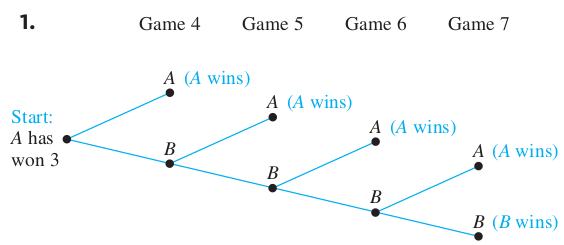
\includegraphics[scale=0.6]{../images/9.2.1.png}
\end{figure}

There are five ways to complete the series: $A$, \(B-A\), \(B-B-A\), \(B-B-B-A\), and \(B-B-B-B\).
\end{proof}

\subsection{Exercise 2}
Suppose team $A$ wins the first two games. How many ways can the World Series be completed? (Draw a tree.)

\begin{proof}
\begin{figure}[ht!]
\centering
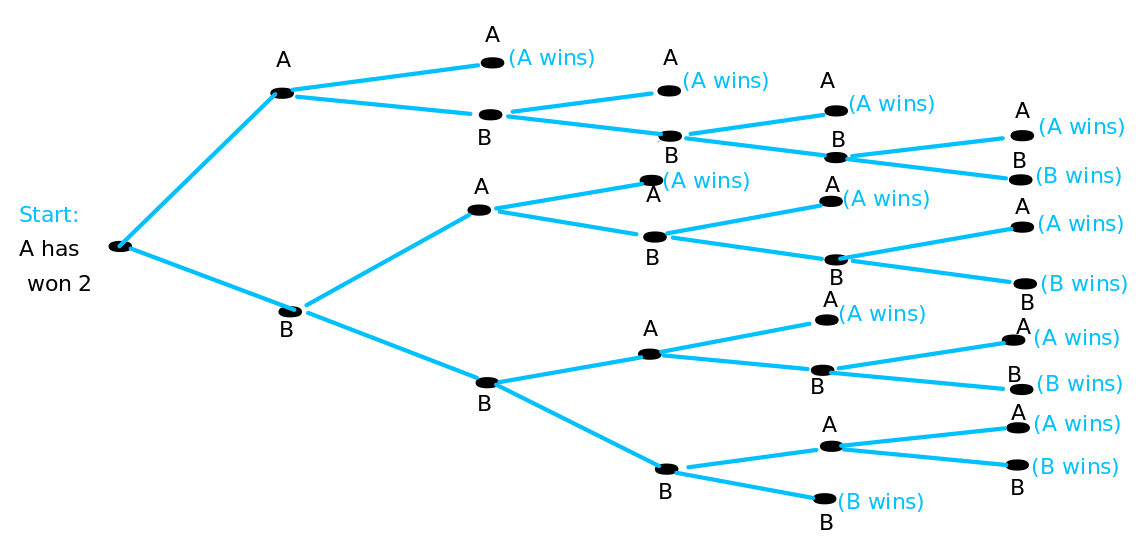
\includegraphics[scale=0.3]{../images/9.2.2.png}
\end{figure}

There are 15 ways: AA, ABA, ABBA, ABBBA, ABBBB, BAA, BABA, BABBA, BABBB, BBAA, BBABA, BBABB, BBBAA, BBBAB, BBBB.
\end{proof}

\subsection{Exercise 3}
How many ways can a World Series be played if team $A$ wins four games in a row?

\begin{proof}
Four ways: \(A-A-A-A, B-A-A-A-A, B-B-A-A-A-A\), and \(B-B-B-A-A-A-A\)
\end{proof}

\subsection{Exercise 4}
How many ways can a World Series be played if no team wins two games in a row?

\begin{proof}
Two ways: \(A-B-A-B-A-B-A\) and \(B-A-B-A-B-A-B\)
\end{proof}

\subsection{Exercise 5}
In a competition between players $X$ and $Y$, the first player to win three games in a row or a total of four games 
wins. How many ways can the competition be played if $X$ wins the first game and $Y$ wins the second and third 
games? (Draw a tree.)

\begin{proof}
\begin{figure}[ht!]
\centering
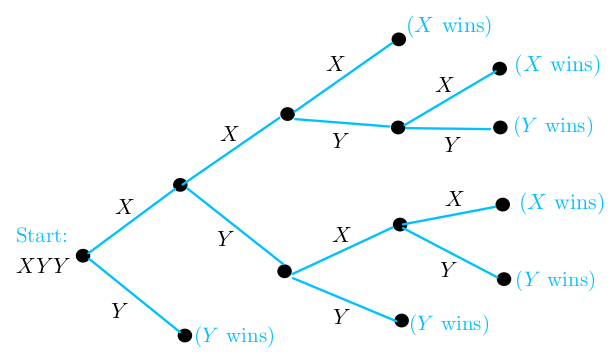
\includegraphics[scale=0.4]{../images/9.2.5.png}
\end{figure}

There are seven ways: \(XXX, XXYX, XXYY, XYXX, XYXY, XYY, Y\).
\end{proof}

\subsection{Exercise 6}
One urn contains two black balls (labeled \(B_1\) and \(B_2\)) and one white ball. A second urn contains one black 
ball and two white balls (labeled \(W_1\) and \(W_2\)). Suppose the following experiment is performed: One of the 
two urns is chosen at random. Next a ball is randomly chosen from the urn. Then a second ball is chosen at random 
from the same urn without replacing the first ball.

\subsubsection{(a)}
Construct the possibility tree showing all possible outcomes of this experiment.

\begin{proof}
\begin{figure}[ht!]
\centering
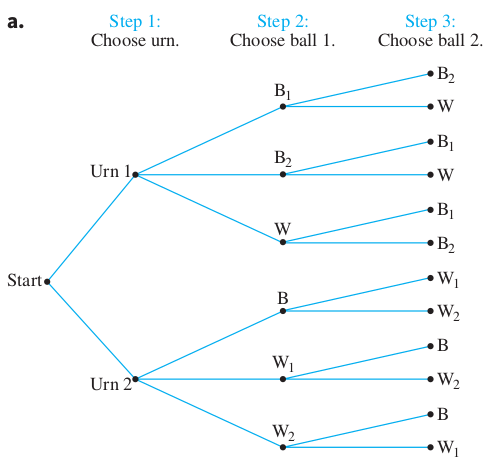
\includegraphics[scale=0.5]{../images/9.2.6.a.png}
\end{figure}
\end{proof}

\subsubsection{(b)}
What is the total number of outcomes of this experiment?

\begin{proof}
12
\end{proof}

\subsubsection{(c)}
What is the probability that two black balls are chosen?

\begin{proof}
\(2/12 = 1/6 \approx 16.6\%\)
\end{proof}

\subsubsection{(d)}
What is the probability that two balls of opposite color are chosen?

\begin{proof}
\(8/12 = 2/3 \approx 66.6\%\)
\end{proof}

\subsection{Exercise 7}
One urn contains one blue ball (labeled \(B_1\)) and three red balls (labeled \(R_1, R_2\), and \(R_3\)). A second urn 
contains two red balls (\(R_4\) and \(R_5\)) and two blue balls (\(B_2\) and \(B_3\)). An experiment is performed in 
which one of the two urns is chosen at random and then two balls are randomly chosen from it, one after the other 
without replacement.

\subsubsection{(a)}
Construct the possibility tree showing all possible outcomes of this experiment.

\begin{proof}
\begin{figure}[ht!]
\centering
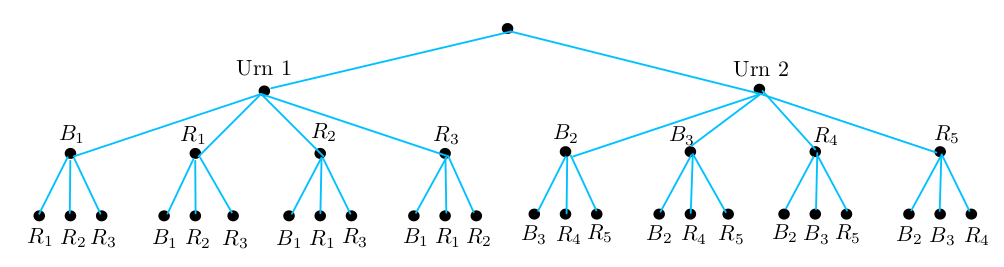
\includegraphics[scale=0.5]{../images/9.2.7.a.png}
\end{figure}
\end{proof}

\subsubsection{(b)}
What is the total number of outcomes of this experiment?

\begin{proof}
24
\end{proof}

\subsubsection{(c)}
What is the probability that two red balls are chosen?

\begin{proof}
\(8/24 = 1/3 \approx 33.3\%\)
\end{proof}

\subsection{Exercise 8}
A person buying a personal computer system is offered a choice of three models of the basic unit, two models of 
keyboard, and two models of printer. How many distinct systems can be purchased?

\begin{proof}
By the multiplication rule, the answer is \(3 \cdot 2 \cdot 2 = 12\).
\end{proof}

\subsection{Exercise 9}
Suppose there are three roads from city $A$ to city $B$ and five roads from city $B$ to city $C$. 

\subsubsection{(a)}
How many ways is it possible to travel from city $A$ to city $C$ via city $B$?

\begin{proof}
In going from city $A$ to city $B$, one may take any of the 3 roads. In going from city $B$ to city $C$, one may take 
any of the 5 roads. So, by the multiplication rule, there are \(3 \cdot 5 = 15\) ways to travel from city $A$ to city 
$C$ via city $B$.
\end{proof}

\subsubsection{(b)}
How many different round-trip routes are there from city $A$ to $B$ to $C$ to $B$ and back to $A$?

\begin{proof}
A round-trip journey can be thought of as a four-step operation: {\cy Step 1:} Go from $A$ to $B$. {\cy Step 2:} 
Go from $B$ to $C$. {\cy Step 3:} Go from $C$ to $B$. {\cy Step 4:} Go from $B$ to $A$.

Since there are 3 ways to perform step 1, 5 ways to perform step 2, 5 ways to perform step 3, and 3 ways to perform 
step 4, by the multiplication rule, there are \(3 \cdot 5 \cdot 5 \cdot 3 = 225\) round-trip routes.
\end{proof}

\subsubsection{(c)}
How many different routes are there from cities $A$ to $B$ to $C$ to $B$ and back to $A$ in which no road is traversed twice?

\begin{proof}
In this case the steps for making a round-trip journey are the same as in part (b), but since no route segment may be 
repeated, there are only 4 ways to perform step 3 and only 2 ways to perform step 4. So, by the multiplication rule, 
there are \(3 \cdot 5 \cdot 4 \cdot 2 = 120\) round-trip routes in which no road is traversed twice.
\end{proof}

\subsection{Exercise 10}
Suppose there are three routes from North Point to Boulder Creek, two routes from Boulder Creek to Beaver Dam, two 
routes from Beaver Dam to Star Lake, and four routes directly from Boulder Creek to Star Lake. (Draw a sketch.)

\subsubsection{(a)}
How many routes from North Point to Star Lake pass through Beaver Dam?

\begin{proof}
By the multiplication rule \(3 \cdot 2 \cdot 2 = 12\) routes.
\end{proof}

\subsubsection{(b)}
How many routes from North Point to Star Lake bypass Beaver Dam?

\begin{proof}
By the multiplication rule \(3 \cdot 4 = 12\) routes.
\end{proof}

\subsection{Exercise 11}
\subsubsection{(a)}
A bit string is a finite sequence of 0’s and 1’s. How many bit strings have length 8?

\begin{proof}
Imagine constructing a bit string of length 8 as an eight-step process:

{\cy Step 1:} Choose either a 0 or a 1 for the left-most position,

{\cy Step 2:} Choose either a 0 or a 1 for the next position to the right.

\(\vdots\)

{\cy Step 8:} Choose either a 0 or a 1 for the right-most position.

Since there are 2 ways to perform each step, the total number of ways to accomplish the entire operation, which is 
the number of different bit strings of length 8, is \(2 \cdot 2 \cdot 2 \cdot 2 \cdot 2 \cdot 2 \cdot 2 \cdot 2 = 
2^8 = 256\).
\end{proof}

\subsubsection{(b)}
How many bit strings of length 8 begin with three 0’s?

\begin{proof}
Imagine that there are three 0’s in the three left-most positions, and imagine filling in the remaining 5 positions 
as a five-step process, where step $i$ is to fill in the \((i + 3)\)rd position. Since there are 2 ways to perform 
each of the 5 steps, there are \(2^5\) ways to perform the entire operation. So there are \(2^5\), or 32, 8-bit 
strings that begin with three 0’s.
\end{proof}

\subsubsection{(c)}
How many bit strings of length 8 begin and end with a 1?

\begin{proof}
\(2^6 = 64\)
\end{proof}

\subsection{Exercise 12}
Hexadecimal numbers are made using the sixteen hexadecimal digits 0, 1, 2, 3, 4, 5, 6, 7, 8, 9, A, B, C, D, E, F and 
are denoted using the subscript 16. For example, 9A2D16 and BC5416 are hexadecimal numbers.

\subsubsection{(a)}
How many hexadecimal numbers begin with one of the digits 3 through B, end with one of the digits 5 through F, and are 
5 digits long?

\begin{proof}
Think of creating a hexadecimal number that satisfies the given requirements as a five-step process. 

{\cy Step 1:} Choose the left-most hexadecimal digits. It can be any of the 9 hexadecimal digits from 3 through B.

{\cy Steps 2-4:} Choose the three hexadecimal digits for the middle three positions. Each can be any of the 16 
hexadecimal digits.

{\cy Step 5:} Choose the right-most hexadecimal digit. It can be any of the 11 hexadecimal digits from 5 through F.

There are 9 ways to perform step 1, 16 ways to perform each of steps 2 through 4, and 11 ways to perform step 5. Thus, 
the total number of specified hexadecimal numbers is \(9 \cdot 16 \cdot 16 \cdot 16 \cdot 11 = 405,504\).
\end{proof}

\subsubsection{(b)}
How many hexadecimal numbers begin with one of the digits 4 through D, end with one of the digits 2 through E, and are 
6 digits long?

\begin{proof}
There are 10 choices for the first digit: 4, 5, 6, 7, 8, 9, A, B, C, D.

There are 14 choices for the first digit: 2, 3, 4, 5, 6, 7, 8, 9, A, B, C, D, E.

There are 16 choices for each one of the 4 middle digits.

So: \(10 \cdot 16 \cdot 16 \cdot 16 \cdot 16 \cdot 14 = 9175040\)
\end{proof}

\subsection{Exercise 13}
A coin is tossed four times. Each time the result H for heads or T for tails is recorded. An outcome of HHTT means that heads were obtained on the first two tosses and tails on the second two. Assume that heads and tails are equally likely on each toss.

\subsubsection{(a)}
How many distinct outcomes are possible?

\begin{proof}
In each of the four tosses there are two possible results: Either a head (H) or a tail (T) is obtained. Thus, by the 
multiplication rule, the number of outcomes is \(2 \cdot 2 \cdot 2 \cdot 2 = 2^4 = 16\).
\end{proof}

\subsubsection{(b)}
What is the probability that exactly two heads occur?

\begin{proof}
There are six outcomes with two heads: HHTT, HTHT, HTTH, THHT, THTH, TTHH. Thus the probability of obtaining exactly 
two heads is \(6/16 = 3/8\).
\end{proof}

\subsubsection{(c)}
What is the probability that exactly one head occurs?

\begin{proof}
There are four outcomes with exactly one head: HTTT, THTT, TTHT, TTTH. Thus the probability of obtaining exactly two 
heads is \(4/16 = 1/4\).
\end{proof}

\subsection{Exercise 14}
Suppose that in a certain state, all automobile license plates have four uppercase letters followed by three 
digits.

\subsubsection{(a)}
How many different license plates are possible?

\begin{proof}
Think of creating license plates that satisfy the given conditions as the following seven-step process: In steps 
1–4 choose the letters to put in positions 1–4, and in steps 5–7, choose the digits to put in positions 5–7. Since 
there are 26 letters and 10 digits and since repetition is allowed, there are 26 ways to perform each of steps 1–4 and 
10 ways to perform each of steps 5–7. Thus the number of license plates is \(26 \cdot 26 \cdot 26 \cdot 26 \cdot 10 
\cdot 10 \cdot 10 = 456,976,000\).
\end{proof}

\subsubsection{(b)}
How many license plates could begin with A and end in 0?
\begin{proof}
In this case there is only one way to perform step 1 (because the first letter must be an A) and only one way to 
perform step 7 (because the last digit must be a 0). Therefore, the number of license plates is 
\(26 \cdot 26 \cdot 26 \cdot 10 \cdot 10 = 1,757,600\).
\end{proof}

\subsubsection{(c)}
How many license plates could begin with TGIF?

\begin{proof}
There are 3 digits left to be chosen. Each has 10 possibilities. So by the multiplication rule \(10^3=1000\)
can begin with TGIF.
\end{proof}

\subsubsection{(d)}
How many license plates are possible in which all the letters and digits are distinct?

\begin{proof}
In this case there are 26 ways to perform step 1, 25 ways to perform step 2, 24 ways to perform step 3, 23 ways to 
perform step 4, 10 ways to perform step 5, 9 ways to perform step 6, and 8 ways to perform step 7, so the number 
of license plates is \(26 \cdot 25 \cdot 24 \cdot 23 \cdot 10 \cdot 9 \cdot 8 = 258,336,000\).
\end{proof}

\subsubsection{(e)}
How many license plates could begin with AB and have all letters and digits distinct?

\begin{proof}
24 choices for the third letter, 23 for the fourth letter. Then 10, 9, 8 choices for the 1st, 2nd, 3rd digits. So:
\(24 \cdot 23 \cdot 10 \cdot 9 \cdot 8 = 397440\).
\end{proof}

\subsection{Exercise 15}
A combination lock requires three selections of numbers, each from 1 through 30.

\subsubsection{(a)}
How many different combinations are possible?

\begin{proof}
\(30^3 = 27000\)
\end{proof}

\subsubsection{(b)}
Suppose the locks are constructed in such a way that no number may be used twice. How many different combinations 
are possible?

\begin{proof}
\(30 \cdot 29 \cdot 28 = 24360\)
\end{proof}

\subsection{Exercise 16}
\subsubsection{(a)}
How many integers are there from 10 through 99?

\begin{proof}
Two solutions:

(i) By the multiplication rule, the number of integers from 10 through 99 = (the number of ways to pick the first 
digit) \(\times\) (the number of ways to pick the second digit) = \(9 \cdot 10 = 90\).

(ii) By Theorem 9.1.1, the number of integers from 10 through 99 = \(90 - 10 + 1 = 90\).
\end{proof}

\subsubsection{(b)}
How many odd integers are there from 10 through 99?

\begin{proof}
Because odd integers end in 1, 3, 5, 7, or 9, the number of odd integers from 10 through 99 = (the number of ways to 
pick the first digit) \(\times\) (the number of ways to pick the second digit) = \(9 \cdot 5 = 45\).

An alternative solution uses the listing method shown in the solution for Example 9.1.4.
\end{proof}

\subsubsection{(c)}
How many integers from 10 through 99 have distinct digits?

\begin{proof}
(the number of ways to pick the first digit) \(\times\) (the number of ways to pick the second digit) = 
\(9 \cdot 9 = 81\).

Another solution is to start with the solution to part (a), which is 90, and subtract the number of integers that have 
the same digit repeated, of which there are 9: 11, 22, 33, 44, 55, 66, 77, 88, 99.
\end{proof}

\subsubsection{(d)}
How many odd integers from 10 through 99 have distinct digits?

\begin{proof}
(the number of ways to pick the second digit) \(\times\) (the number of ways to pick the first digit) = \(5 \cdot 8 
= 40\). Here the second digit can be 1,3,5,7,9; and the first digit cannot be 0 or the same as the first digit.
\end{proof}

\subsubsection{(e)}
What is the probability that a randomly chosen two-digit integer has distinct digits? has distinct digits and is odd?

\begin{proof}
81/90 = 9/10, 40/90 = 4/9
\end{proof}

\subsection{Exercise 17}
\subsubsection{(a)}
How many integers are there from 1000 through 9999?

\begin{proof}
By Theorem 9.1.1, \(9999-1000+1 = 9000\). Another solution: there are 9 choices for the first digit (cannot be 0), and
10 choices for the other 3 digits, so \(9 \cdot 10 \cdot 10 \cdot 10 = 9000\).
\end{proof}

\subsubsection{(b)}
How many odd integers are there from 1000 through 9999?

\begin{proof}
4500.

One solution is that it's half of the answer to part (a), since half the integers are even, and the other odd. 

Another solution: there are 9 choices for the first digit (cannot be 0), 10 choices for the second and third digits,
and 5 choices for the last (1,3,5,7,9), therefore \(9 \cdot 10 \cdot 10 \cdot 5 = 4500\).
\end{proof}

\subsubsection{(c)}
How many integers from 1000 through 9999 have distinct digits?

\begin{proof}
There are 9 choices for the first digit (cannot be 0). There are 9 choices for the second digit (cannot be the same as the first digit, but can be 0). Then 8 and 7 choices for the third and fourth digits. So there are  
\(9 \cdot 9 \cdot 8 \cdot 7 = 4536\) such integers.
\end{proof}

\subsubsection{(d)}
How many odd integers from 1000 through 9999 have distinct digits?

\begin{proof}
There are 5 choices for the last digit (1, 3, 5, 7, 9). There are 8 choices for the first digit (cannot be the 
same as the last digit, and cannot be 0). Then 8 choices for the second digit (cannot be the same as the first or 
the last, but can be 0) and 7 choices for the third digit. So there are \(5 \cdot 8 \cdot 8 \cdot 7 = 2240\) such 
integers.
\end{proof}

\subsubsection{(e)}
What is the probability that a randomly chosen four-digit integer has distinct digits? has distinct digits and is odd?

\begin{proof}
4536/9000, 2240/9000
\end{proof}

\subsection{Exercise 18}
The following diagram shows the keypad for an automatic teller machine. As you can see, the same sequence of keys 
represents a variety of different PINs. For instance, 2133, AZDE, and BQ3F are all keyed in exactly the same way.

\begin{figure}[ht!]
\centering
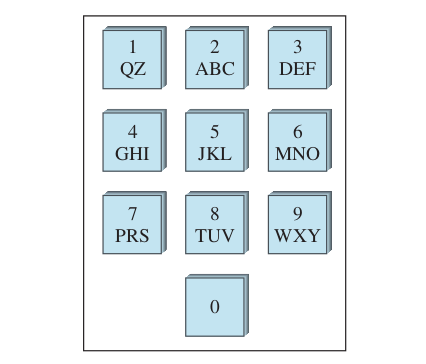
\includegraphics[scale=0.5]{../images/9.2.18.png}
\end{figure}

\subsubsection{(a)}
How many different PINs are represented by the same sequence of keys as 2133?

\begin{proof}
Let step 1 be to choose either the number 2 or one of the letters corresponding to the number 2 on the keypad, let 
step 2 be to choose either the number 1 or one of the letters corresponding to the number 1 on the keypad, and 
let steps 3 and 4 be to choose either the number 3 or one of the letters corresponding to the number 3 on the keypad. 
There are 4 ways to perform step 1, 3 ways to perform step 2, and 4 ways to perform each of steps 3 and 4. So by the 
multiplication rule, there are \(4 \cdot 3 \cdot 4 \cdot 4 = 192\) ways to perform the entire operation. Thus there 
are 192 different PINs that are keyed the same as 2133. Note that on a computer keyboard, these PINs would not be 
keyed the same way.
\end{proof}

\subsubsection{(b)}
How many different PINs are represented by the same sequence of keys as 5031?

\begin{proof}
\(4 \cdot 1 \cdot 4 \cdot 3 = 48\)
\end{proof}

\subsubsection{(c)}
How many different numeric sequences on the machine contain no repeated digit?

\begin{proof}
\(10 \cdot 9 \cdot 8 \cdot 7 = 5040\)
\end{proof}

\subsection{Exercise 19}
Three officers - a president, a treasurer, and a secretary - are to be chosen from among four people: Ann, Bob, Cyd, 
and Dan. Suppose that Bob is not qualified to be treasurer and Cyd’s other commitments make it impossible for her to 
be secretary. How many ways can the officers be chosen? Can the multiplication rule be used to solve this problem?

\begin{proof}
There are 14 different paths from “root” to “leaf” of this possibility tree, and so there are 14 ways the officers can 
be chosen. Because \(14 = 2\cdot7\), reordering the steps will not make it possible to use the multiplication rule 
alone to solve this problem.

\begin{figure}[ht!]
\centering
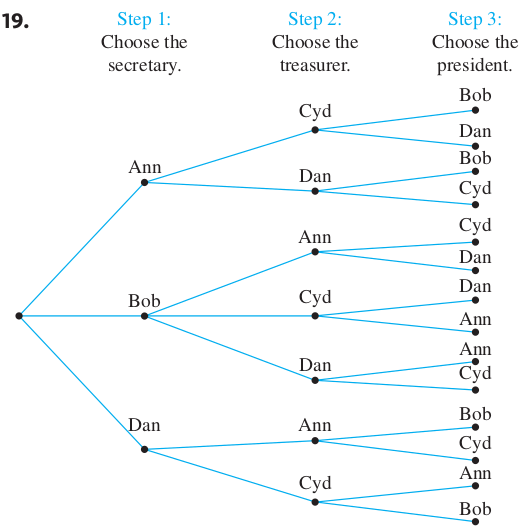
\includegraphics[scale=0.45]{../images/9.2.19.png}
\end{figure}
\end{proof}

\subsection{Exercise 20}
Modify Example 9.2.2 by supposing that a PIN must not begin with any of the letters A-M and must end with a digit. Continue to assume that no symbol may be used more than once and that the total number of PINs is to be determined.

\subsubsection{(a)}
Find the error in the following “solution.” “Constructing a PIN is a four-step process. 

Step 1: Choose the left-most symbol.

Step 2: Choose the second symbol from the left.

Step 3: Choose the third symbol from the left.

Step 4: Choose the right-most symbol.

Because none of the thirteen letters from A through M may be chosen in step 1, there are \(36 - 13 = 23\) ways to 
perform step 1. There are 35 ways to perform step 2 and 34 ways to perform step 3 because previously used symbols may 
not be used. Since the symbol chosen in step 4 must be a previously unused digit, there are \(10 - 3 = 7\) ways to 
perform step 4. Thus there are \(23 \cdot 35 \cdot 34 \cdot 7 = 191,590\) different PINs that satisfy the given 
conditions.”

\begin{proof}
The number of ways to perform step 4 is not constant; it depends on how the previous steps were performed. For 
instance, if 3 digits had been chosen in steps 1-3, then there would be \(10 - 3 = 7\) ways to perform step 4, but 
if 3 letters had been chosen in steps 1-3, then there would be 10 ways to perform step 4.
\end{proof}

\subsubsection{(b)}
Reorder steps 1-4 in part (a) as follows: {\cy Step 1:} Choose the right-most symbol. {\cy Step 2:} Choose the 
left-most symbol. {\cy Step 3:} Choose the second symbol from the left. {\cy Step 4:} Choose the third symbol from 
the left. Use the multiplication rule to find the number of PINs that satisfy the given conditions.

\begin{proof}
\(10 \cdot 22 \cdot 34 \cdot 33 = 246840\)
\end{proof}

\subsection{Exercise 21}
Suppose $A$ is a set with $m$ elements and $B$ is a set with $n$ elements.

\subsubsection{(a)}
How many relations are there from $A$ to $B$? Explain.

\begin{proof}
\(2^{mn}\). There are $mn$ pairs in \(A \times B\). A relation is simply any subset of \(A \times B\). So the
number of relations from $A$ to $B$ is the same as the size of the power set of \(A \times B\), which is \(2^{mn}\).
\end{proof}

\subsubsection{(b)}
How many functions are there from $A$ to $B$? Explain.

\begin{proof}
\(n^m\). For each input \(a \in A\) there are $n$ possible outputs \(b \in B\). Since there are $m$ inputs, by the
multiplication rule there are \(n \cdot n \cdots n = n^m\) functions.
\end{proof}

\subsubsection{(c)}
What fraction of the relations from $A$ to $B$ are functions?

\begin{proof}
\(n^m / 2^{mn}\)
\end{proof}

\subsection{Exercise 22}
\subsubsection{(a)}
How many functions are there from a set with three elements to a set with four elements?

\begin{proof}
The answer is \(4 \cdot 4 \cdot 4 = 4^3 = 64\). Imagine creating a function from a 3-element set to a 4-element set 
as a three-step process: Step 1 is to send the first element of the 3-element set to an element of the 4-element 
set (there are four ways to perform this step); step 2 is to send the second element of the 3-element set to an 
element of the 4-element set (there are also four ways to perform this step); and step 3 is to send the third element 
of the 3-element set to an element of the 4-element set (there are four ways to perform this step). Thus the entire 
process can be performed in \(4 \cdot 4 \cdot 4\) different ways.
\end{proof}

\subsubsection{(b)}
How many functions are there from a set with five elements to a set with two elements?

\begin{proof}
\(2^5 = 32\)
\end{proof}

\subsubsection{(c)}
How many functions are there from a set with $m$ elements to a set with $n$ elements, where $m$ and $n$ are positive 
integers?

\begin{proof}
\(n^m\).
\end{proof}

\subsection{Exercise 23}
In Section 2.5 we showed how integers can be represented by strings of 0’s and 1’s inside a digital computer. In fact, 
through various coding schemes, strings of 0’s and 1’s can be used to represent all kinds of symbols. One commonly 
used code is the Extended Binary-Coded Decimal Interchange Code (EBCDIC) in which each symbol has an 8-bit 
representation. How many distinct symbols can be represented by this code?

\begin{proof}
\(2^8 = 256\)
\end{proof}

{\bf \cy In each of $24-28$, determine how many times the innermost loop will be iterated when the algorithm segment 
is implemented and run. (assume that \(m, n, p, a, b, c\), and $d$ are all positive integers.)}

\subsection{Exercise 24}
\begin{tabbing}
{\bf for} \= \(i \coloneqq 1\) {\bf to} 30 \\
          \> {\bf for} \= \(j \coloneqq 1\) {\bf to} 15 \\
          \>           \> {\it [Statements in body of inner loop.]} \\
          \>           \> {\it [None contain branching statements that lead outside the loop.]} \\
          \> {\bf next j} \\
{\bf next i}
\end{tabbing}

\begin{proof}
The outer loop is iterated 30 times, and during each iteration of the outer loop there are 15 iterations of the 
inner loop. Hence, by the multiplication rule, the total number of iterations of the inner loop is 
\(30 \cdot 15 = 450\).
\end{proof}

\subsection{Exercise 25}
\begin{tabbing}
{\bf for} \= \(j \coloneqq 1\) {\bf to} $m$ \\
          \> {\bf for} \= \(k \coloneqq 1\) {\bf to} $n$ \\
          \>           \> {\it [Statements in body of inner loop.]} \\
          \>           \> {\it [None contain branching statements that lead outside the loop.]} \\
          \> {\bf next k} \\
{\bf next j}
\end{tabbing}

\begin{proof}
\(mn\)
\end{proof}

\subsection{Exercise 26}
\begin{tabbing}
{\bf for} \= \(i \coloneqq 1\) {\bf to} $m$ \\
          \> {\bf for} \= \(j \coloneqq 1\) {\bf to} $n$ \\
          \>           \> {\bf for} \= \(k \coloneqq 1\) {\bf to} $p$ \\
          \>           \>           \> {\it [Statements in body of inner loop.]} \\
          \>           \>           \> {\it [None contain branching statements that lead outside the loop.]} \\
          \>           \> {\bf next k} \\
          \> {\bf next j} \\
{\bf next i}
\end{tabbing}

\begin{proof}
\(mnp\)
\end{proof}

\subsection{Exercise 27}
\begin{tabbing}
{\bf for} \= \(i \coloneqq 5\) {\bf to} 50 \\
          \> {\bf for} \= \(j \coloneqq 10\) {\bf to} 20 \\
          \>           \> {\it [Statements in body of inner loop.]} \\
          \>           \> {\it [None contain branching statements that lead outside the loop.]} \\
          \> {\bf next j} \\
{\bf next i}
\end{tabbing}

\begin{proof}
The outer loop is iterated \(50 - 5 + 1 = 46\) times, and during each iteration of the outer loop there are 
\(20 - 10 + 1 = 11\) iterations of the inner loop. Hence, by the multiplication rule, the total number of iterations 
of the inner loop is \(46 \cdot 11 = 506\).
\end{proof}

\subsection{Exercise 28}
Assume \(a \leq b\) and \(c \leq d\).
\begin{tabbing}
{\bf for} \= \(i \coloneqq a\) {\bf to} $b$ \\
          \> {\bf for} \= \(j \coloneqq c\) {\bf to} $d$ \\
          \>           \> {\it [Statements in body of inner loop.]} \\
          \>           \> {\it [None contain branching statements that lead outside the loop.]} \\
          \> {\bf next j} \\
{\bf next i}
\end{tabbing}

\begin{proof}
\((b-a+1)(d-c+1)\)
\end{proof}

\subsection{Exercise 29}
Consider the numbers 1 through 99,999 in their ordinary decimal representations. How many contain exactly one of 
each of the digits 2, 3, 4, and 5?

{\it Hint:} An efficient solution is to add leading zeros as needed to make each number five digits long. For 
instance, write 1 as 00001. Then, instead of choosing digits for the positions, choose positions for the digits. 
The answer is 720.

\begin{proof}
Following the Hint, there are 5 possible positions to place 2, then 4 positions to place 3, 3 positions to place 4, 2
positions to place 5, and 6 choices for the last position (1, 6, 7, 8, 9, 0). Therefore \(5 \cdot 4 \cdot 3 \cdot 2
\cdot 6 = 720\). (Notice that there is no issue with the digit 0, since it can be placed in the first position.)
\end{proof}

\subsection{Exercise 30}
Let \(n = p_1^{k_1} p_2^{k_2} \cdots p_m^{k_m}\) where \(p_1, p_2, \ldots, p_m\) are distinct prime numbers and 
\(k_1, k_2, \ldots, k_m\) are positive integers. How many ways can $n$ be written as a product of two positive 
integers that have no common factors, assuming the following?

\subsubsection{(a)}
Order matters (that is, \(8 \cdot 15\) and \(15 \cdot 8\) are regarded as different).

\begin{proof}
To split $n$ into two positive integers $a, b$ that have no common factors, we need to split the set of all the prime 
powers \(\{p_1^{k_1}, \cdots, p_m^{k_m}\) into two disjoint subsets $A, B$. Then $a$ is the product of the prime powers in $A$, and $b$ is the product of those in $B$.

When one of the subsets is chosen, the other is automatically forced to be what's left. For example, if the
set is \(p_1^{k_1}, p_2^{k_2}, p_3^{k_3}\) and we choose $A$ to be \(\{p_1^{k_1}, p_3^{k_3}\}\) then $B$ has to be
\(\{p_2^{k_2}\}\).

However, since order matters, choosing $A$ to be \(\{p_1^{k_1}, p_3^{k_3}\}\) and $B$ to be \(\{p_2^{k_2}\}\) 
is considered different than choosing $A$ to be \(\{p_2^{k_2}\}\) and $B$ to be \(\{p_1^{k_1}, p_3^{k_3}\}\).

This means that the number of ways to write $n$ as the product of two positive integers with no common prime 
factors is equal to the number of ways we can choose $A$ to be a subset of \(\{p_1^{k_1}, \ldots, p_m^{k_m}\}\). This 
is a set with $m$ elements, so it has $2^m$ subsets. So there are $2^m$ ways to choose $A$, which is the answer.
\end{proof}

\subsubsection{(b)}
Order does not matter (that is, \(8 \cdot 15\) and \(15 \cdot 8\) are regarded as the same).

\begin{proof}
The solution is the same as in part (a) except the choices where $A$ and $B$ are swapped do not count. For example, 
choosing $A$ to be \(\{p_1^{k_1}, p_3^{k_3}\}\) and $B$ to be \(\{p_2^{k_2}\}\) is considered the same as choosing $A$ 
to be \(\{p_2^{k_2}\}\) and $B$ to be \(\{p_1^{k_1}, p_3^{k_3}\}\).

So, in this case the answer is half the answer to part (a), namely, \(2^m / 2 = 2^{m-1}\).
\end{proof}

\subsection{Exercise 31}
\subsubsection{(a)}
If $p$ is a prime number and $a$ is a positive integer, how many distinct positive divisors does $p^a$ have?

\begin{proof}
There are \(a + 1\) divisors: \(1, p, p^2, \ldots, p^a\).
\end{proof}

\subsubsection{(b)}
If $p$ and $q$ are distinct prime numbers and $a$ and $b$ are positive integers, how many distinct positive divisors 
does $p^a q^b$ have?

\begin{proof}
A divisor is a product of any one of the \(a + 1\) numbers listed in part (a) times any one of the \(b + 1\) numbers 
\(1, q, q^2, \ldots, q^b\). So, by the multiplication rule, there are \((a + 1)(b + 1)\) divisors in all.
\end{proof}

\subsubsection{(c)}
If $p, q$, and $r$ are distinct prime numbers and $a, b$, and $c$ are positive integers, how many distinct positive 
divisors does $p^a q^b r^c$ have?

\begin{proof}
\((a+1)(b+1)(c+1)\)
\end{proof}

\subsubsection{(d)}
If \(p_1, p_2, \ldots, p_m\) are distinct prime numbers and \(a_1, a_2, \ldots, a_m\) are positive integers, how many 
distinct positive divisors does \(p_1^{a_1} p_2^{a_2} \cdots p_m^{a_m}\) have?

\begin{proof}
\((a_1+1)(a_2+1) \cdots (a_m+1)\)
\end{proof}

\subsubsection{(e)}
What is the smallest positive integer with exactly 12 divisors?

\begin{proof}
Assume \(p_1, p_2, \ldots, p_m\) are distinct prime numbers and \(a_1, a_2, \ldots, a_m\) are positive integers, and 
\(n = p_1^{a_1} p_2^{a_2} \cdots p_m^{a_m}\) is the integer we are looking for. Assume $n$ has exactly 12 divisors.

By part (d), \(12 = 2 \cdot 2 \cdot 3\) so $m=3$ and \(2 \cdot 2 \cdot 3 = (a_1+1)(a_2+1)(a_3+1)\) so it follows 
\(a_1 = 1, a_2 = 1, a_3 = 2\). 

To make $n$ as small as possible, we can choose the smallest first three primes 2, 3, 5, and since \(a_3 = 2\) 
we can let \(p_1 = 3, p_2 = 5, p_3 = 2\). (This way the highest power 2 goes on top of the smallest base prime, 2.)

Therefore \(n = p_1^{a_1} p_2^{a_2} p_3^{a_3} = 3^1 \cdot 5^1 \cdot 2^2 = 60\) is the smallest positive integer with 
exactly 12 divisors: 1, 2, 3, 4, 5, 6, 10, 12, 15, 20, 30, 60.
\end{proof}

\subsection{Exercise 32}
\subsubsection{(a)}
How many ways can the letters of the word ALGORITHM be arranged in a row?

\begin{proof}
Since the nine letters of the word ALGORITHM are all distinct, there are as many arrangements of these letters 
in a row as there are permutations of a set with nine elements: \(9! = 362,880\).
\end{proof}

\subsubsection{(b)}
How many ways can the letters of the word ALGORITHM be arranged in a row if A and L must remain together (in 
order) as a unit?

\begin{proof}
In this case there are effectively eight symbols to be permuted (because AL may be regarded as a single symbol). 
So the number of arrangements is \(8! = 40,320\).
\end{proof}

\subsubsection{(c)}
How many ways can the letters of the word ALGORITHM be arranged in a row if the letters GOR must remain together 
(in order) as a unit?

\begin{proof}
In this case there are effectively seven symbols to be permuted (because GOR may be regarded as a single symbol). 
So the number of arrangements is \(7! = 5040\).
\end{proof}

\subsection{Exercise 33}
Six people attend the theater together and sit in a row with exactly six seats.

\subsubsection{(a)}
How many ways can they be seated together in the row?

\begin{proof}
\(6! = 720\)
\end{proof}

\subsubsection{(b)}
Suppose one of the six is a doctor who must sit on the aisle in case she is paged. How many ways can the people be 
seated together in the row with the doctor in an aisle seat?

\begin{proof}
Excluding the doctor who must sit on the aisle seat, \(5! = 120\) ways. (However the question is a bit ambiguous, are 
there 2 aisle seats, one on each side of the row? In that case the answer would be 240.)
\end{proof}

\subsubsection{(c)}
Suppose the six people consist of three married couples and each couple wants to sit together with the older partner on 
the left. How many ways can the six be seated together in the row?

\begin{proof}
The couples can be treated as one person, so \(3! = 6\).
\end{proof}

\subsection{Exercise 34}
Five people are to be seated around a circular table. Two seatings are considered the same if one is a rotation of 
the other. How many different seatings are possible?

\begin{proof}
The same reasoning as in Example 9.2.9 gives an answer of \(4! = 24\).
\end{proof}

\subsection{Exercise 35}
Write all the 2-permutations of \(\{W, X, Y, Z\}\).

\begin{proof}
\(WX, WY, WZ, XW, XY, XZ, YW, YX, YZ, ZW, ZX, ZY\)
\end{proof}

\subsection{Exercise 36}
Write all the 3-permutations of \(\{s, t, u, v\}\).

\begin{proof}
There are \(P(4,3) = \dps\frac{4!}{(4-3)!} = 24\) 3-permutations of a 4-element set. So:

\(stu, stv, suv, sut, svt, svu, tsu, tsv, tuv, tus, tvs, tvu,\)

\(ust, usv, utv, uts, uvs, uvt, vst, vsu, vtu, vts, vus, vut.\)
\end{proof}

\subsection{Exercise 37}
Evaluate the following quantities.

\subsubsection{(a)}
\(P(6, 4)\)
\begin{proof}
\(P(6,4) = \dps\frac{6!}{(6-4)!} = \frac{6!}{2!} = \frac{6 \cdot 5 \cdot 4 \cdot 3 \cdot \Ccancel[cyan]{2 \cdot 1}}
{\Ccancel[cyan]{2 \cdot 1}} = 360\)
\end{proof}

\subsubsection{(b)}
\(P(6, 6)\)
\begin{proof}
\(P(6,6) = \dps\frac{6!}{(6-6)!} = \frac{6!}{0!} = 720/1 = 720\)
\end{proof}

\subsubsection{(c)}
\(P(6, 3)\)
\begin{proof}
\(P(6,3) = \dps\frac{6!}{(6-3)!} = \frac{6!}{3!} = \frac{6 \cdot 5 \cdot 4 \cdot \Ccancel[cyan]{3 \cdot 2 \cdot 1}}
{\Ccancel[cyan]{3 \cdot 2 \cdot 1}} = 120\)
\end{proof}

\subsubsection{(d)}
\(P(6, 1)\)
\begin{proof}
\(P(6,1) = \dps\frac{6!}{(6-1)!} = \frac{6!}{5!} = \frac{6 \cdot \Ccancel[cyan]{5 \cdot 4 \cdot 3 \cdot 2 \cdot 1}}
{\Ccancel[cyan]{5 \cdot 4 \cdot 3 \cdot 2 \cdot 1}} = 6\)
\end{proof}

\subsection{Exercise 38}
\subsubsection{(a)}
How many 3-permutations are there of a set of five objects?

\begin{proof}
\(P(5,3) = \dps\frac{5!}{(5-3)!} = \frac{5!}{2!} = \frac{5 \cdot 4 \cdot 3 \cdot \Ccancel[cyan]{2 \cdot 1}}
{\Ccancel[cyan]{2 \cdot 1}} = 60\)
\end{proof}

\subsubsection{(b)}
How many 2-permutations are there of a set of eight objects?

\begin{proof}
\(P(8,2) = \dps\frac{8!}{(8-2)!} = \frac{8!}{6!} = \frac{8 \cdot 7 \cdot \Ccancel[cyan]{6 \cdot 5 \cdot 4 \cdot 3 
\cdot 2 \cdot 1}}{\Ccancel[cyan]{6 \cdot 5 \cdot 4 \cdot 3 
\cdot 2 \cdot 1}} = 56\)
\end{proof}

\subsection{Exercise 39}
\subsubsection{(a)}
How many ways can three of the letters of the word ALGORITHM be selected and written in a row?

\begin{proof}
\(P(9,3) = \dps\frac{9!}{(9-3)!} = \frac{9!}{6!} = \frac{9 \cdot 8 \cdot 7 \cdot \Ccancel[cyan]{6!}}
{\Ccancel[cyan]{6!}} = 504\)
\end{proof}

\subsubsection{(b)}
How many ways can six of the letters of the word ALGORITHM be selected and written in a row?

\begin{proof}
\(P(9,6) = \dps\frac{9!}{(9-6)!} = \frac{9!}{3!} = \frac{9 \cdot 8 \cdot 7 \cdot 6 \cdot 5 \cdot 4 \cdot 
\Ccancel[cyan]{3!}}{\Ccancel[cyan]{3!}} = 60480\)
\end{proof}

\subsubsection{(c)}
How many ways can six of the letters of the word ALGORITHM be selected and written in a row if the first letter must be A?

\begin{proof}
\(P(8,5) = \dps\frac{8!}{(8-5)!} = \frac{8!}{3!} = \frac{8 \cdot 7 \cdot 6 \cdot 5 \cdot 4 \cdot \Ccancel[cyan]{3!}}
{\Ccancel[cyan]{3!}} = 6720\)
\end{proof}

\subsubsection{(d)}
How many ways can six of the letters of the word ALGORITHM be selected and written in a row if the first two letters must be OR?

\begin{proof}
\(P(7,4) = \dps\frac{7!}{(7-4)!} = \frac{7!}{3!} = \frac{7 \cdot 6 \cdot 5 \cdot 4 \cdot \Ccancel[cyan]{3!}}
{\Ccancel[cyan]{3!}} = 840\)
\end{proof}

\subsection{Exercise 40}
Prove that for every integer \(n \geq 2\), \(P(n + 1, 3) = n^3 - n\).

\begin{proof}
\(P(n+1,3) = \dps\frac{(n+1)!}{(n+1-3)!} = \frac{(n+1)!}{(n-2)!} = \frac{(n+1) \cdot n \cdot (n-1) \cdot 
\Ccancel[cyan]{(n-2)!}}{\Ccancel[cyan]{(n-2)!}}\)

\(= (n+1)n(n-1) = (n^2-1)n = n^3-n\)
\end{proof}

\subsection{Exercise 41}
Prove that for every integer \(n \geq 2\), \(P(n + 1, 2) - P(n, 2) = 2P(n, 1)\).

\begin{proof}
\(P(n+1,2) = \dps\frac{(n+1)!}{(n+1-2)!} = \frac{(n+1)!}{(n-1)!} = \frac{(n+1) \cdot n!}{(n-1)!} = (n+1)P(n,1)\)

\(P(n,2) = \dps\frac{n!}{(n-2)!} = \frac{(n-1) \cdot n!}{(n-1) \cdot (n-2)!} = (n-1)\frac{n!}{(n-1)!}=(n-1)P(n,1)\)

So \(P(n + 1, 2) - P(n, 2) = (n+1)P(n, 1) - (n-1)P(n, 1) = 2P(n,1)\).
\end{proof}

\subsection{Exercise 42}
Prove that for every integer \(n \geq 3\), \(P(n + 1, 3) - P(n, 3) = 3P(n, 2)\).

\begin{proof}
\(P(n+1,3) = \dps\frac{(n+1)!}{(n+1-3)!} = \frac{(n+1)!}{(n-2)!} = \frac{(n+1) \cdot n!}{(n-2)!} = (n+1)P(n,2)\)

\(P(n,3) = \dps\frac{n!}{(n-3)!} = \frac{(n-2) \cdot n!}{(n-2) \cdot (n-3)!} = (n-2)\frac{n!}{(n-2)!}=(n-2)P(n,2)\)

So \(P(n + 1, 3) - P(n, 3) = (n+1)P(n, 2) - (n-2)P(n, 2) = 3P(n,2)\).
\end{proof}

\subsection{Exercise 43}
Prove that for every integer \(n \geq 2\), \(P(n, n) = P(n, n - 1)\).

\begin{proof}
\(P(n,n)= \dps\frac{n!}{(n-n)!} = \frac{n!}{0!} = \frac{n!}{1} = \frac{n!}{1!} = \frac{n!}{(n-(n-1))!} = P(n,n-1)\)
\end{proof}

\subsection{Exercise 44}
Prove Theorem 9.2.1 by mathematical induction.

\begin{proof}
Let \(P(k)\) be the statement: ``If an operation consists of $k$ steps and the first step can be performed in $n_1$ 
ways, the second step can be performed in $n_2$ ways {\it [regardless of how the first step was performed]}, 
\(\ldots\), the $k$th step can be performed in $n_k$ ways {\it [regardless of how the preceding steps were 
performed]}, then the entire operation can be performed in \(n_1n_2 \cdots n_k\) ways.''

{\bf Show that \(P(1)\) is true:} Assume an operation consists of 1 step, and the first step can be performed in
\(n_1\) ways. Then the whole operation can be performed in \(n_1\) ways, so \(P(1)\) is true.

{\bf Show that for any integer \(k \geq 1\) if \(P(k)\) is true then \(P(k+1)\) is true:} Assume an operation consists
of $k+1$ steps, and assume steps \(1, 2, 3, \ldots, k+1\) can be performed in \(n_1, n_2, \ldots, n_{k+1}\) ways,
respectively, regardless of how preceding steps are performed. Assume that the first $k$ steps can be performed 
in \(n_1n_2 \cdots n_k\) ways. {\it [This is the inductive hypothesis.]}

Since the $k+1$st step can be performed in \(n_{k+1}\) ways regardless of how the preceding $k$ steps were performed, 
for each way of performing the preceding $k$ steps, there are \(n_{k+1}\) ways to perform step $k+1$. Thus there are
\[
\underbrace{n_{k+1} + n_{k+1} + \cdots + n_{k+1}}_{n_1n_2 \cdots n_k \text{ times}}
\]
ways to perform the whole task, where the sum has \(n_1n_2 \cdots n_k\) terms. And the sum equals
\[
n_{k+1} \cdot (n_1n_2 \cdots n_k) = n_1n_2 \cdots n_k n_{k+1}
\]
{\it [as was to be shown.]}
\end{proof}

\subsection{Exercise 45}
Prove Theorem 9.2.2 by mathematical induction.

\begin{proof}
Let \(P(n)\) be the statement ``For any integer $n$ with \(n \geq 1\), the number of permutations of a set with $n$ 
elements is \(n!\).''

{\bf Show that \(P(1)\) is true:} There is only 1 permutation of a set with 1 element, and \(1! = 1\), so 
\(P(1)\) is true.

{\bf Show that for any integer \(k \geq 1\) if \(P(k)\) is true then \(P(k+1)\) is true:} Assume \(k \geq 1\) and 
assume that the number of permutations of any set with $k$ elements is $k!$. {\it [This is the inductive hypothesis.]}
Assume \(A = \{a_1, \ldots, a_{k+1}\}\) is a set with $k+1$ elements.

Consider the subset \(A' = \{a_1, \ldots, a_k\}\) of $A$ with $k$ elements. By the inductive hypothesis $A'$ has 
$k!$ permutations. Now we need to find a way to write the permutations of $A$ in terms of the permutations of $A'$.

Every permutation of $A$ can be thought of as taking a permutation of $A$ and then inserting \(a_{k+1}\) into a
position in that permutation. For example, if \(a_3, a_1, a_{k-2}, \ldots, a_k, a_2, a_{k-1}\) is a permutation of 
$A'$, then there are $k+1$ positions in which \(a_{k+1}\) can be inserted to obtain a permutation of $A$:
\begin{center}
\begin{tabular}{ccccccccccccccc}
& \(a_3\) & & \(a_1\) & & \(a_{k-2}\) & & \(\ldots\) & & \(a_k\) & & \(a_2\) & & \(a_{k-1}\) & \\
\(\uparrow\) & & \(\uparrow\) & & \(\uparrow\) & & \(\uparrow\)& \(\ldots\) & \(\uparrow\) & & \(\uparrow\)& &\(\uparrow\)& & \(\uparrow\) \\
here & & here & & here & & here& \(\ldots\) & here & & here& &here& & here \\
\end{tabular}
\end{center}
So for each permutation of $A'$, there are $k+1$ permutations of $A$. Therefore the number of permutations 
of $A$ is \(k! \cdot (k+1) = (k+1)!\).
\end{proof}

\subsection{Exercise 46}
Prove Theorem 9.2.3 by mathematical induction.

\begin{proof}
Let \(Q(n)\) be the statement: ``for every integer $r$ with \(1 \leq r \leq n\), 
\(P(n,r) = n(n - 1)(n - 2) \cdots (n - r + 1)\).''

{\bf Show that \(Q(1)\) is true:} There is only one 1-permutation of a set of 1 element, and when \(n=r=1\)
the formula \(n(n - 1)(n - 2) \cdots (n - r + 1)\) is equal to 1. Therefore \(Q(1)\) is true.

{\bf Show that for any integer \(k \geq 1\) if \(Q(k)\) is true then \(Q(k+1)\) is true:} Assume \(k \geq 1\) and 
assume for every integer $r$ with \(1 \leq r \leq k\), \(P(k,r) = k(k - 1)(k - 2) \cdots (k - r + 1)\). 
{\it [This is the inductive hypothesis.]}

We want to show that for every integer $r$ with \(1 \leq r \leq k+1\), \(P(k+1,r) = (k+1)k(k-1) \cdots (k-r + 2)\).

When \(r = 1\), there are $k+1$ ways to choose 1 element from a set of $k+1$ elements. So \(P(k+1,1) = k+1\), and
the formula \((k+1)k(k-1) \cdots (k-r + 2)\) for \(r = 1\) becomes \((k+1)\), therefore the formula holds.

Now assume \(2 \leq r \leq k+1\). We can think of choosing $r$ elements from a set of $k+1$ elements as follows: first
choosing 1 element out of $k+1$ elements, then choosing $r-1$ elements from the remaining $k$ elements.

There are $k+1$ ways to choose the first element. Then by the inductive hypothesis there are \(P(k, r-1) = k(k - 1)
(k - 2) \cdots (k - (r-1) + 1) = k(k - 1)(k - 2) \cdots (k - r + 2)\) ways to choose $r-1$ elements from the remaining
$k$ elements. Then by the multiplication rule, \(P(k+1,r) = (k+1) \cdot k(k - 1)(k - 2) \cdots (k - r + 2)\), 
{\it [as was to be shown.]}
\end{proof}

\subsection{Exercise 47}
A permutation on a set can be regarded as a function from the set to itself. For instance, one permutation of 
\(\{1, 2, 3, 4\}\) is 2341. It can be identified with the function that sends each position number to the number 
occupying that position. Since position 1 is occupied by 2, 1 is sent to 2 or \(1 \to 2\); since position 2 is occupied 
by 3, 2 is sent to 3 or \(2 \to 3\); and so forth. The entire permutation can be written using arrows as follows:

\begin{center}
\begin{tabular}{cccc}
1&2&3&4 \\
\cyda & \cyda & \cyda & \cyda \\
2&3&4&1 \\
\end{tabular}
\end{center}

\subsubsection{(a)}
Use arrows to write each of the six permutations of \(\{1, 2, 3\}\).

\begin{proof}
\begin{center}
\begin{tabular}{ccc|ccc|ccc|ccc|ccc|ccc}
1&2&3&1&2&3&1&2&3&1&2&3&1&2&3&1&2&3 \\
\cyda & \cyda & \cyda & \cyda & \cyda & \cyda & \cyda & \cyda & \cyda & \cyda & \cyda & \cyda & \cyda & \cyda & 
\cyda & \cyda & \cyda & \cyda \\
1&2&3&1&3&2&2&1&3&2&3&1&3&1&2&3&2&1
\end{tabular}
\end{center}
\end{proof}

\subsubsection{(b)}
Use arrows to write each of the permutations of \(\{1, 2, 3, 4\}\) that keep 2 and 4 fixed.

\begin{proof}
\begin{center}
\begin{tabular}{cccc|cccc}
1&2&3&4&1&2&3&4 \\
\cyda & \cyda & \cyda & \cyda & \cyda & \cyda & \cyda & \cyda \\
1&2&3&4&3&2&1&4
\end{tabular}
\end{center}
\end{proof}

\subsubsection{(c)}
Which permutations of \(\{1, 2, 3\}\) keep no elements fixed?

\begin{proof}
\begin{center}
\begin{tabular}{ccc|ccc}
1&2&3&1&2&3 \\
\cyda & \cyda & \cyda & \cyda & \cyda & \cyda \\
2&3&1&3&1&2 \\
\end{tabular}
\end{center}
\end{proof}

\subsubsection{(d)}
Use arrows to write all permutations of \(\{1, 2, 3, 4\}\) that keep no elements fixed.

\begin{proof}
\begin{center}
\begin{tabular}{cccc|cccc|cccc|cccc|cccc|cccc}
1&2&3&4&1&2&3&4&1&2&3&4&1&2&3&4&1&2&3&4&1&2&3&4 \\
\cyda & \cyda & \cyda & \cyda & \cyda & \cyda & \cyda & \cyda & \cyda & \cyda & \cyda & \cyda & \cyda & \cyda & 
\cyda & \cyda & \cyda & \cyda & \cyda & \cyda & \cyda & \cyda & \cyda & \cyda \\
2&1&4&3&2&3&4&1&2&4&1&3&3&1&4&2&3&4&1&2&3&4&2&1
\end{tabular}
\end{center}
\begin{center}
\begin{tabular}{cccc|cccc|cccc}
1&2&3&4&1&2&3&4&1&2&3&4\\
\cyda & \cyda & \cyda & \cyda & \cyda & \cyda & \cyda & \cyda & \cyda & \cyda & \cyda & \cyda \\
4&1&2&3&4&3&1&2&4&3&2&1
\end{tabular}
\end{center}
\end{proof}

\section{Exercise Set 9.3}

\subsection{Exercise 1}

\subsubsection{(a)}

\begin{proof}

\end{proof}

\subsubsection{(b)}

\begin{proof}

\end{proof}

\subsection{Exercise 2}

\subsubsection{(a)}

\begin{proof}

\end{proof}

\subsubsection{(b)}

\begin{proof}

\end{proof}

\subsection{Exercise 3}

\subsubsection{(a)}

\begin{proof}

\end{proof}

\subsubsection{(b)}

\begin{proof}

\end{proof}

\subsubsection{(c)}

\begin{proof}

\end{proof}

\subsection{Exercise 4}

\begin{proof}

\end{proof}

\subsection{Exercise 5}

\subsubsection{(a)}

\begin{proof}

\end{proof}

\subsubsection{(b)}

\begin{proof}

\end{proof}

\subsection{Exercise 6}

\subsubsection{(a)}

\begin{proof}

\end{proof}

\subsubsection{(b)}

\begin{proof}

\end{proof}

\subsubsection{(c)}

\begin{proof}

\end{proof}

\subsubsection{(d)}

\begin{proof}

\end{proof}

\subsection{Exercise 7}

\subsubsection{(a)}

\begin{proof}

\end{proof}

\subsubsection{(b)}

\begin{proof}

\end{proof}

\subsubsection{(c)}

\begin{proof}

\end{proof}

\subsubsection{(d)}

\begin{proof}

\end{proof}

\subsection{Exercise 8}

\subsubsection{(a)}

\begin{proof}

\end{proof}

\subsubsection{(b)}

\begin{proof}

\end{proof}

\subsubsection{(c)}

\begin{proof}

\end{proof}

\subsubsection{(d)}

\begin{proof}

\end{proof}

\subsection{Exercise 9}

\subsubsection{(a)}

\begin{proof}

\end{proof}

\subsubsection{(b)}

\begin{proof}

\end{proof}

\subsection{Exercise 10}

\begin{proof}

\end{proof}

\subsection{Exercise 11}
\subsubsection{(a)}

\begin{proof}

\end{proof}

\subsubsection{(b)}

\begin{proof}

\end{proof}

\subsubsection{(c)}

\begin{proof}

\end{proof}

\subsection{Exercise 12}

\subsubsection{(a)}

\begin{proof}

\end{proof}

\subsubsection{(b)}

\begin{proof}

\end{proof}

\subsection{Exercise 13}

\subsubsection{(a)}

\begin{proof}

\end{proof}

\subsubsection{(b)}

\begin{proof}

\end{proof}

\subsection{Exercise 14}

\begin{proof}

\end{proof}

\subsection{Exercise 15}

\begin{proof}

\end{proof}

\subsection{Exercise 16}

\subsubsection{(a)}

\begin{proof}

\end{proof}

\subsubsection{(b)}

\begin{proof}

\end{proof}

\subsubsection{(c)}

\begin{proof}

\end{proof}

\subsection{Exercise 17}
\subsubsection{(a)}

\begin{proof}

\end{proof}

\subsubsection{(b)}

\begin{proof}

\end{proof}

\subsubsection{(c)}

\begin{proof}

\end{proof}

\subsection{Exercise 18}

\subsubsection{(a)}

\begin{proof}

\end{proof}

\subsubsection{(b)}

\begin{proof}

\end{proof}

\subsection{Exercise 19}

\begin{proof}

\end{proof}

\subsection{Exercise 20}

\subsubsection{(a)}

\begin{proof}

\end{proof}

\subsubsection{(b)}

\begin{proof}

\end{proof}

\subsubsection{(c)}

\begin{proof}

\end{proof}

\subsection{Exercise 21}

\begin{proof}

\end{proof}

\subsection{Exercise 22}

\subsubsection{(a)}

\begin{proof}

\end{proof}

\subsubsection{(b)}

\begin{proof}

\end{proof}

\subsection{Exercise 23}

\subsubsection{(a)}

\begin{proof}

\end{proof}

\subsubsection{(b)}

\begin{proof}

\end{proof}

\subsubsection{(c)}

\begin{proof}

\end{proof}

\subsection{Exercise 24}

\subsubsection{(a)}

\begin{proof}

\end{proof}

\subsubsection{(b)}

\begin{proof}

\end{proof}

\subsubsection{(c)}

\begin{proof}

\end{proof}

\subsection{Exercise 25}

\subsubsection{(a)}

\begin{proof}

\end{proof}

\subsubsection{(b)}

\begin{proof}

\end{proof}

\subsubsection{(c)}

\begin{proof}

\end{proof}

\subsubsection{(d)}

\begin{proof}

\end{proof}

\subsection{Exercise 26}

\subsubsection{(a)}

\begin{proof}

\end{proof}

\subsubsection{(b)}

\begin{proof}

\end{proof}

\subsubsection{(c)}

\begin{proof}

\end{proof}

\subsubsection{(d)}

\begin{proof}

\end{proof}

\subsubsection{(e)}

\begin{proof}

\end{proof}

\subsection{Exercise 27}

\subsubsection{(a)}

\begin{proof}

\end{proof}

\subsubsection{(b)}

\begin{proof}

\end{proof}

\subsection{Exercise 28}

\subsubsection{(a)}

\begin{proof}

\end{proof}

\subsubsection{(b)}

\begin{proof}

\end{proof}

\subsection{Exercise 29}

\subsubsection{(a)}

\begin{proof}

\end{proof}

\subsubsection{(b)}

\begin{proof}

\end{proof}

\subsubsection{(c)}

\begin{proof}

\end{proof}

\subsubsection{(d)}

\begin{proof}

\end{proof}

\subsubsection{(e)}

\begin{proof}

\end{proof}

\subsubsection{(f)}

\begin{proof}

\end{proof}

\subsubsection{(g)}

\begin{proof}

\end{proof}

\subsubsection{(h)}

\begin{proof}

\end{proof}

\subsubsection{(i)}

\begin{proof}

\end{proof}

\subsubsection{(j)}

\begin{proof}

\end{proof}

\subsection{Exercise 30}

\begin{proof}

\end{proof}

\subsection{Exercise 31}

\subsubsection{(a)}

\begin{proof}

\end{proof}

\subsubsection{(b)}

\begin{proof}

\end{proof}

\subsubsection{(c)}

\begin{proof}

\end{proof}

\subsubsection{(d)}

\begin{proof}

\end{proof}

\subsubsection{(e)}

\begin{proof}

\end{proof}

\subsection{Exercise 32}

\begin{proof}

\end{proof}

\subsection{Exercise 33}

\subsubsection{(a)}

\begin{proof}

\end{proof}

\subsubsection{(b)}

\begin{proof}

\end{proof}

\subsubsection{(c)}

\begin{proof}

\end{proof}

\subsubsection{(d)}

\begin{proof}

\end{proof}

\subsubsection{(e)}

\begin{proof}

\end{proof}

\subsubsection{(f)}

\begin{proof}

\end{proof}

\subsection{Exercise 34}

\subsubsection{(a)}

\begin{proof}

\end{proof}

\subsubsection{(b)}

\begin{proof}

\end{proof}

\subsubsection{(c)}

\begin{proof}

\end{proof}

\subsubsection{(d)}

\begin{proof}

\end{proof}

\subsection{Exercise 35}

\begin{proof}

\end{proof}

\subsection{Exercise 36}

\begin{proof}

\end{proof}

\subsection{Exercise 37}

\begin{proof}

\end{proof}

\subsection{Exercise 38}

\begin{proof}

\end{proof}

\subsection{Exercise 39}

\begin{proof}

\end{proof}

\subsection{Exercise 40}

\begin{proof}

\end{proof}

\subsection{Exercise 41}

\begin{proof}

\end{proof}

\subsection{Exercise 42}

\subsubsection{(a)}

\begin{proof}

\end{proof}

\subsubsection{(b)}

\begin{proof}

\end{proof}

\subsubsection{(c)}

\begin{proof}

\end{proof}

\subsection{Exercise 43}

\subsubsection{(a)}

\begin{proof}

\end{proof}

\subsubsection{(b)}

\begin{proof}

\end{proof}

\subsubsection{(c)}

\begin{proof}

\end{proof}

\subsection{Exercise 44}

\begin{proof}

\end{proof}

\subsection{Exercise 45}

\begin{proof}

\end{proof}

\subsection{Exercise 46}

\begin{proof}

\end{proof}

\subsection{Exercise 47}

\begin{proof}

\end{proof}

\subsection{Exercise 48}

\begin{proof}

\end{proof}

\subsection{Exercise 49}

\subsubsection{(a)}

\begin{proof}

\end{proof}

\subsubsection{(b)}

\begin{proof}

\end{proof}

\section{Exercise Set 9.4}

\subsection{Exercise 1}

\subsubsection{(a)}

\begin{proof}

\end{proof}

\subsubsection{(b)}

\begin{proof}

\end{proof}

\subsection{Exercise 2}

\subsubsection{(a)}

\begin{proof}

\end{proof}

\subsubsection{(b)}

\begin{proof}

\end{proof}

\subsection{Exercise 3}

\begin{proof}

\end{proof}

\subsection{Exercise 4}

\begin{proof}

\end{proof}

\subsection{Exercise 5}

\subsubsection{(a)}

\begin{proof}

\end{proof}

\subsubsection{(b)}

\begin{proof}

\end{proof}

\subsection{Exercise 6}

\subsubsection{(a)}

\begin{proof}

\end{proof}

\subsubsection{(b)}

\begin{proof}

\end{proof}

\subsection{Exercise 7}

\begin{proof}

\end{proof}

\subsection{Exercise 8}

\begin{proof}

\end{proof}

\subsection{Exercise 9}

\subsubsection{(a)}

\begin{proof}

\end{proof}

\subsubsection{(b)}

\begin{proof}

\end{proof}

\subsection{Exercise 10}

\begin{proof}

\end{proof}

\subsection{Exercise 11}

\begin{proof}

\end{proof}

\subsection{Exercise 12}

\begin{proof}

\end{proof}

\subsection{Exercise 13}

\begin{proof}

\end{proof}

\subsection{Exercise 14}

\begin{proof}

\end{proof}

\subsection{Exercise 15}

\begin{proof}

\end{proof}

\subsection{Exercise 16}

\begin{proof}

\end{proof}

\subsection{Exercise 17}

\begin{proof}

\end{proof}

\subsection{Exercise 18}

\begin{proof}

\end{proof}

\subsection{Exercise 19}

\begin{proof}

\end{proof}

\subsection{Exercise 20}

\subsubsection{(a)}

\begin{proof}

\end{proof}

\subsubsection{(b)}

\begin{proof}

\end{proof}

\subsection{Exercise 21}

\begin{proof}

\end{proof}

\subsection{Exercise 22}

\begin{proof}

\end{proof}

\subsection{Exercise 23}

\begin{proof}

\end{proof}

\subsection{Exercise 24}

\begin{proof}

\end{proof}

\subsection{Exercise 25}

\begin{proof}

\end{proof}

\subsection{Exercise 26}

\begin{proof}

\end{proof}

\subsection{Exercise 27}

\begin{proof}

\end{proof}

\subsection{Exercise 28}

\begin{proof}

\end{proof}

\subsection{Exercise 29}

\begin{proof}

\end{proof}

\subsection{Exercise 30}

\begin{proof}

\end{proof}

\subsection{Exercise 31}

\begin{proof}

\end{proof}

\subsection{Exercise 32}

\begin{proof}

\end{proof}

\subsection{Exercise 33}

\begin{proof}

\end{proof}

\subsection{Exercise 34}

\begin{proof}

\end{proof}

\subsection{Exercise 35}

\begin{proof}

\end{proof}

\subsection{Exercise 36}

\begin{proof}

\end{proof}

\subsection{Exercise 37}
\subsubsection{(a)}

\begin{proof}

\end{proof}

\subsubsection{(b)}

\begin{proof}

\end{proof}

\subsection{Exercise 38}

\begin{proof}

\end{proof}

\subsection{Exercise 39}

\begin{proof}

\end{proof}

\subsection{Exercise 40}

\begin{proof}

\end{proof}

\section{Exercise Set 9.5}

\subsection{Exercise 1}

\subsubsection{(a)}

\begin{proof}

\end{proof}

\subsubsection{(b)}

\begin{proof}

\end{proof}

\subsection{Exercise 2}

\subsubsection{(a)}

\begin{proof}

\end{proof}

\subsubsection{(b)}

\begin{proof}

\end{proof}

\subsection{Exercise 3}

\begin{proof}

\end{proof}

\subsection{Exercise 4}

\begin{proof}

\end{proof}

\subsection{Exercise 5}

\subsubsection{(a)}

\begin{proof}

\end{proof}

\subsubsection{(b)}

\begin{proof}

\end{proof}

\subsubsection{(c)}

\begin{proof}

\end{proof}

\subsubsection{(d)}

\begin{proof}

\end{proof}

\subsubsection{(e)}

\begin{proof}

\end{proof}

\subsection{Exercise 6}

\subsubsection{(a)}

\begin{proof}

\end{proof}

\subsubsection{(b)}

\begin{proof}

\end{proof}

\subsubsection{(c)}

\begin{proof}

\end{proof}

\subsubsection{(d)}

\begin{proof}

\end{proof}

\subsubsection{(e)}

\begin{proof}

\end{proof}

\subsection{Exercise 7}

\subsubsection{(a)}

\begin{proof}

\end{proof}

\subsubsection{(b)}

\begin{proof}

\end{proof}

\subsubsection{(c)}

\begin{proof}

\end{proof}

\subsubsection{(d)}

\begin{proof}

\end{proof}

\subsection{Exercise 8}

\subsubsection{(a)}

\begin{proof}

\end{proof}

\subsubsection{(b)}

\begin{proof}

\end{proof}

\subsubsection{(c)}

\begin{proof}

\end{proof}

\subsubsection{(d)}

\begin{proof}

\end{proof}

\subsection{Exercise 9}

\subsubsection{(a)}

\begin{proof}

\end{proof}

\subsubsection{(b)}

\begin{proof}

\end{proof}

\subsection{Exercise 10}

\begin{proof}

\end{proof}

\subsection{Exercise 11}

\subsubsection{(a)}

\begin{proof}

\end{proof}

\subsubsection{(b)}

\begin{proof}

\end{proof}

\subsubsection{(c)}

\begin{proof}

\end{proof}

\subsubsection{(d)}

\begin{proof}

\end{proof}

\subsubsection{(e)}

\begin{proof}

\end{proof}

\subsubsection{(f)}

\begin{proof}

\end{proof}

\subsubsection{(g)}

\begin{proof}

\end{proof}

\subsubsection{(h)}

\begin{proof}

\end{proof}

\subsubsection{(i)}

\begin{proof}

\end{proof}

\subsection{Exercise 12}

\begin{proof}

\end{proof}

\subsection{Exercise 13}

\subsubsection{(a)}

\begin{proof}

\end{proof}

\subsubsection{(b)}

\begin{proof}

\end{proof}

\subsubsection{(c)}

\begin{proof}

\end{proof}

\subsubsection{(d)}

\begin{proof}

\end{proof}

\subsubsection{(e)}

\begin{proof}

\end{proof}

\subsection{Exercise 14}

\subsubsection{(a)}

\begin{proof}

\end{proof}

\subsubsection{(b)}

\begin{proof}

\end{proof}

\subsubsection{(c)}

\begin{proof}

\end{proof}

\subsubsection{(d)}

\begin{proof}

\end{proof}

\subsection{Exercise 15}

\subsubsection{(a)}

\begin{proof}

\end{proof}

\subsubsection{(b)}

\begin{proof}

\end{proof}

\subsubsection{(c)}

\begin{proof}

\end{proof}

\subsubsection{(d)}

\begin{proof}

\end{proof}

\subsection{Exercise 16}

\subsubsection{(a)}

\begin{proof}

\end{proof}

\subsubsection{(b)}

\begin{proof}

\end{proof}

\subsubsection{(c)}

\begin{proof}

\end{proof}

\subsection{Exercise 17}

\subsubsection{(a)}

\begin{proof}

\end{proof}

\subsubsection{(b)}

\begin{proof}

\end{proof}

\subsubsection{(c)}

\begin{proof}

\end{proof}

\subsubsection{(d)}

\begin{proof}

\end{proof}

\subsection{Exercise 18}

\begin{proof}

\end{proof}

\subsection{Exercise 19}

\subsubsection{(a)}

\begin{proof}

\end{proof}

\subsubsection{(b)}

\begin{proof}

\end{proof}

\subsubsection{(c)}

\begin{proof}

\end{proof}

\subsection{Exercise 20}

\subsubsection{(a)}

\begin{proof}

\end{proof}

\subsubsection{(b)}

\begin{proof}

\end{proof}

\subsubsection{(c)}

\begin{proof}

\end{proof}

\subsection{Exercise 21}

\begin{proof}

\end{proof}

\subsection{Exercise 22}

\begin{proof}

\end{proof}

\subsection{Exercise 23}

\begin{proof}

\end{proof}

\subsection{Exercise 24}

\subsubsection{(a)}

\begin{proof}

\end{proof}

\subsubsection{(b)}

\begin{proof}

\end{proof}

\subsubsection{(c)}

\begin{proof}

\end{proof}

\subsubsection{(d)}

\begin{proof}

\end{proof}

\subsection{Exercise 25}

\subsubsection{(a)}

\begin{proof}

\end{proof}

\subsubsection{(b)}

\begin{proof}

\end{proof}

\subsubsection{(c)}

\begin{proof}

\end{proof}

\subsubsection{(d)}

\begin{proof}

\end{proof}

\subsubsection{(e)}

\begin{proof}

\end{proof}

\subsection{Exercise 26}

\subsubsection{(a)}

\begin{proof}

\end{proof}

\subsubsection{(b)}

\begin{proof}

\end{proof}

\subsubsection{(c)}

\begin{proof}

\end{proof}

\subsubsection{(d)}

\begin{proof}

\end{proof}

\subsubsection{(e)}

\begin{proof}

\end{proof}

\subsubsection{(f)}

\begin{proof}

\end{proof}

\subsection{Exercise 27}

\subsubsection{(a)}

\begin{proof}

\end{proof}

\subsubsection{(b)}

\begin{proof}

\end{proof}

\subsubsection{(c)}

\begin{proof}

\end{proof}

\subsubsection{(d)}

\begin{proof}

\end{proof}

\subsection{Exercise 28}

\begin{proof}

\end{proof}

\subsection{Exercise 29}

\begin{proof}

\end{proof}

\subsection{Exercise 30}

\begin{proof}

\end{proof}

\section{Exercise Set 9.6}

\subsection{Exercise 1}

\subsubsection{(a)}

\begin{proof}

\end{proof}

\subsubsection{(b)}

\begin{proof}

\end{proof}

\subsection{Exercise 2}

\subsubsection{(a)}

\begin{proof}

\end{proof}

\subsubsection{(b)}

\begin{proof}

\end{proof}

\subsection{Exercise 3}

\subsubsection{(a)}

\begin{proof}

\end{proof}

\subsubsection{(b)}

\begin{proof}

\end{proof}

\subsubsection{(c)}

\begin{proof}

\end{proof}

\subsection{Exercise 4}

\subsubsection{(a)}

\begin{proof}

\end{proof}

\subsubsection{(b)}

\begin{proof}

\end{proof}

\subsubsection{(c)}

\begin{proof}

\end{proof}

\subsection{Exercise 5}

\begin{proof}

\end{proof}

\subsection{Exercise 6}

\begin{proof}

\end{proof}

\subsection{Exercise 7}

\begin{proof}

\end{proof}

\subsection{Exercise 8}

\begin{proof}

\end{proof}

\subsection{Exercise 9}

\begin{proof}

\end{proof}

\subsection{Exercise 10}

\begin{proof}

\end{proof}

\subsection{Exercise 11}

\begin{proof}

\end{proof}

\subsection{Exercise 12}

\begin{proof}

\end{proof}

\subsection{Exercise 13}

\begin{proof}

\end{proof}

\subsection{Exercise 14}

\begin{proof}

\end{proof}

\subsection{Exercise 15}

\begin{proof}

\end{proof}

\subsection{Exercise 16}

\subsubsection{(a)}

\begin{proof}

\end{proof}

\subsubsection{(b)}

\begin{proof}

\end{proof}

\subsubsection{(c)}

\begin{proof}

\end{proof}

\subsection{Exercise 17}

\subsubsection{(a)}

\begin{proof}

\end{proof}

\subsubsection{(b)}

\begin{proof}

\end{proof}

\subsubsection{(c)}

\begin{proof}

\end{proof}

\subsubsection{(d)}

\begin{proof}

\end{proof}

\subsection{Exercise 18}

\subsubsection{(a)}

\begin{proof}

\end{proof}

\subsubsection{(b)}

\begin{proof}

\end{proof}

\subsubsection{(c)}

\begin{proof}

\end{proof}

\subsubsection{(d)}

\begin{proof}

\end{proof}

\subsection{Exercise 19}

\subsubsection{(a)}

\begin{proof}

\end{proof}

\subsubsection{(b)}

\begin{proof}

\end{proof}

\subsection{Exercise 20}

\subsubsection{(a)}

\begin{proof}

\end{proof}

\subsubsection{(b)}

\begin{proof}

\end{proof}

\subsection{Exercise 21}

\begin{proof}

\end{proof}

\section{Exercise Set 9.7}

\subsection{Exercise 1}

\begin{proof}

\end{proof}

\subsection{Exercise 2}

\begin{proof}

\end{proof}

\subsection{Exercise 3}

\begin{proof}

\end{proof}

\subsection{Exercise 4}

\begin{proof}

\end{proof}

\subsection{Exercise 5}

\begin{proof}

\end{proof}

\subsection{Exercise 6}

\begin{proof}

\end{proof}

\subsection{Exercise 7}

\begin{proof}

\end{proof}

\subsection{Exercise 8}

\begin{proof}

\end{proof}

\subsection{Exercise 9}

\begin{proof}

\end{proof}

\subsection{Exercise 10}

\subsubsection{(a)}

\begin{proof}

\end{proof}

\subsubsection{(b)}

\begin{proof}

\end{proof}

\subsubsection{(c)}

\begin{proof}

\end{proof}

\subsection{Exercise 11}

\begin{proof}

\end{proof}

\subsection{Exercise 12}

\begin{proof}

\end{proof}

\subsection{Exercise 13}

\begin{proof}

\end{proof}

\subsection{Exercise 14}

\begin{proof}

\end{proof}

\subsection{Exercise 15}

\begin{proof}

\end{proof}

\subsection{Exercise 16}

\begin{proof}

\end{proof}

\subsection{Exercise 17}

\begin{proof}

\end{proof}

\subsection{Exercise 18}

\begin{proof}

\end{proof}

\subsection{Exercise 19}

\begin{proof}

\end{proof}

\subsection{Exercise 20}

\begin{proof}

\end{proof}

\subsection{Exercise 21}

\begin{proof}

\end{proof}

\subsection{Exercise 22}

\begin{proof}

\end{proof}

\subsection{Exercise 23}

\begin{proof}

\end{proof}

\subsection{Exercise 24}

\begin{proof}

\end{proof}

\subsection{Exercise 25}

\begin{proof}

\end{proof}

\subsection{Exercise 26}

\begin{proof}

\end{proof}

\subsection{Exercise 27}

\begin{proof}

\end{proof}

\subsection{Exercise 28}

\begin{proof}

\end{proof}

\subsection{Exercise 29}

\begin{proof}

\end{proof}

\subsection{Exercise 30}

\begin{proof}

\end{proof}

\subsection{Exercise 31}

\begin{proof}

\end{proof}

\subsection{Exercise 32}

\begin{proof}

\end{proof}

\subsection{Exercise 33}

\begin{proof}

\end{proof}

\subsection{Exercise 34}

\begin{proof}

\end{proof}

\subsection{Exercise 35}

\begin{proof}

\end{proof}

\subsection{Exercise 36}

\begin{proof}

\end{proof}

\subsection{Exercise 37}

\begin{proof}

\end{proof}

\subsection{Exercise 38}

\begin{proof}

\end{proof}

\subsection{Exercise 39}

\begin{proof}

\end{proof}

\subsection{Exercise 40}

\begin{proof}

\end{proof}

\subsection{Exercise 41}

\begin{proof}

\end{proof}

\subsection{Exercise 42}

\begin{proof}

\end{proof}

\subsection{Exercise 43}

\begin{proof}

\end{proof}

\subsection{Exercise 44}

\begin{proof}

\end{proof}

\subsection{Exercise 45}

\begin{proof}

\end{proof}

\subsection{Exercise 46}

\begin{proof}

\end{proof}

\subsection{Exercise 47}

\begin{proof}

\end{proof}

\subsection{Exercise 48}

\begin{proof}

\end{proof}

\subsection{Exercise 49}

\begin{proof}

\end{proof}

\subsection{Exercise 50}

\begin{proof}

\end{proof}

\subsection{Exercise 51}

\begin{proof}

\end{proof}

\subsection{Exercise 52}

\begin{proof}

\end{proof}

\subsection{Exercise 53}

\begin{proof}

\end{proof}

\subsection{Exercise 54}

\begin{proof}

\end{proof}

\subsection{Exercise 55}

\subsubsection{(a)}

\begin{proof}

\end{proof}

\subsubsection{(b)}

\begin{proof}

\end{proof}

\subsubsection{(c)}

\begin{proof}

\end{proof}

\subsubsection{(d)}

\begin{proof}

\end{proof}

\section{Exercise Set 9.8}

\subsection{Exercise 1}

\begin{proof}

\end{proof}

\subsection{Exercise 2}

\begin{proof}

\end{proof}

\subsection{Exercise 3}

\subsubsection{(a)}

\begin{proof}

\end{proof}

\subsubsection{(b)}

\begin{proof}

\end{proof}

\subsection{Exercise 4}

\begin{proof}

\end{proof}

\subsection{Exercise 5}

\begin{proof}

\end{proof}

\subsection{Exercise 6}

\begin{proof}

\end{proof}

\subsection{Exercise 7}

\subsubsection{(a)}

\begin{proof}

\end{proof}

\subsubsection{(b)}

\begin{proof}

\end{proof}

\subsubsection{(c)}

\begin{proof}

\end{proof}

\subsubsection{(d)}

\begin{proof}

\end{proof}

\subsubsection{(e)}

\begin{proof}

\end{proof}

\subsubsection{(f)}

\begin{proof}

\end{proof}

\subsection{Exercise 8}

\begin{proof}

\end{proof}

\subsection{Exercise 9}

\subsubsection{(a)}

\begin{proof}

\end{proof}

\subsubsection{(b)}

\begin{proof}

\end{proof}

\subsubsection{(c)}

\begin{proof}

\end{proof}

\subsubsection{(d)}

\begin{proof}

\end{proof}

\subsubsection{(e)}

\begin{proof}

\end{proof}

\subsubsection{(f)}

\begin{proof}

\end{proof}

\subsection{Exercise 10}

\begin{proof}

\end{proof}

\subsection{Exercise 11}

\begin{proof}

\end{proof}

\subsection{Exercise 12}

\begin{proof}

\end{proof}

\subsection{Exercise 13}

\begin{proof}

\end{proof}

\subsection{Exercise 14}

\begin{proof}

\end{proof}

\subsection{Exercise 15}

\begin{proof}

\end{proof}

\subsection{Exercise 16}

\begin{proof}

\end{proof}

\subsection{Exercise 17}

\begin{proof}

\end{proof}

\subsection{Exercise 18}

\begin{proof}

\end{proof}

\subsection{Exercise 19}

\begin{proof}

\end{proof}

\subsection{Exercise 20}

\begin{proof}

\end{proof}

\subsection{Exercise 21}

\begin{proof}

\end{proof}

\subsection{Exercise 22}

\begin{proof}

\end{proof}

\subsection{Exercise 23}

\begin{proof}

\end{proof}

\section{Exercise Set 9.9}

\subsection{Exercise 1}

\begin{proof}

\end{proof}

\subsection{Exercise 2}

\begin{proof}

\end{proof}

\subsection{Exercise 3}

\begin{proof}

\end{proof}

\subsection{Exercise 4}

\subsubsection{(a)}

\begin{proof}

\end{proof}

\subsubsection{(b)}

\begin{proof}

\end{proof}

\subsection{Exercise 5}

\begin{proof}

\end{proof}

\subsection{Exercise 6}

\subsubsection{(a)}

\begin{proof}

\end{proof}

\subsubsection{(b)}

\begin{proof}

\end{proof}

\subsubsection{(c)}

\begin{proof}

\end{proof}

\subsection{Exercise 7}

\begin{proof}

\end{proof}

\subsection{Exercise 8}

\subsubsection{(a)}

\begin{proof}

\end{proof}

\subsubsection{(b)}

\begin{proof}

\end{proof}

\subsubsection{(c)}

\begin{proof}

\end{proof}

\subsection{Exercise 9}

\begin{proof}

\end{proof}

\subsection{Exercise 10}

\begin{proof}

\end{proof}

\subsection{Exercise 11}

\subsubsection{(a)}

\begin{proof}

\end{proof}

\subsubsection{(b)}

\begin{proof}

\end{proof}

\subsection{Exercise 12}

\begin{proof}

\end{proof}

\subsection{Exercise 13}

\subsubsection{(a)}

\begin{proof}

\end{proof}

\subsubsection{(b)}

\begin{proof}

\end{proof}

\subsection{Exercise 14}

\subsubsection{(a)}

\begin{proof}

\end{proof}

\subsubsection{(b)}

\begin{proof}

\end{proof}

\subsection{Exercise 15}

\subsubsection{(a)}

\begin{proof}

\end{proof}

\subsubsection{(b)}

\begin{proof}

\end{proof}

\subsubsection{(c)}

\begin{proof}

\end{proof}

\subsubsection{(d)}

\begin{proof}

\end{proof}

\subsection{Exercise 16}

\subsubsection{(a)}

\begin{proof}

\end{proof}

\subsubsection{(b)}

\begin{proof}

\end{proof}

\subsection{Exercise 17}

\begin{proof}

\end{proof}

\subsection{Exercise 18}

\begin{proof}

\end{proof}

\subsection{Exercise 19}

\begin{proof}

\end{proof}

\subsection{Exercise 20}

\begin{proof}

\end{proof}

\subsection{Exercise 21}

\begin{proof}

\end{proof}

\subsection{Exercise 22}

\begin{proof}

\end{proof}

\subsection{Exercise 23}

\subsubsection{(a)}

\begin{proof}

\end{proof}

\subsubsection{(b)}

\begin{proof}

\end{proof}

\subsubsection{(c)}

\begin{proof}

\end{proof}

\subsection{Exercise 24}

\subsubsection{(a)}

\begin{proof}

\end{proof}

\subsubsection{(b)}

\begin{proof}

\end{proof}

\subsection{Exercise 25}

\subsubsection{(a)}

\begin{proof}

\end{proof}

\subsubsection{(b)}

\begin{proof}

\end{proof}

\subsubsection{(c)}

\begin{proof}

\end{proof}

\subsubsection{(d)}

\begin{proof}

\end{proof}

\subsection{Exercise 26}

\begin{proof}

\end{proof}

\subsection{Exercise 27}

\begin{proof}

\end{proof}

\subsection{Exercise 28}

\subsubsection{(a)}

\begin{proof}

\end{proof}

\subsubsection{(b)}

\begin{proof}

\end{proof}

\subsubsection{(c)}

\begin{proof}

\end{proof}

\subsubsection{(d)}

\begin{proof}

\end{proof}

\subsection{Exercise 29}

\subsubsection{(a)}

\begin{proof}

\end{proof}

\subsubsection{(b)}

\begin{proof}

\end{proof}

\subsubsection{(c)}

\begin{proof}

\end{proof}

\subsubsection{(d)}

\begin{proof}

\end{proof}

\subsection{Exercise 30}

\subsubsection{(a)}

\begin{proof}

\end{proof}

\subsubsection{(b)}

\begin{proof}

\end{proof}

\subsubsection{(c)}

\begin{proof}

\end{proof}

\subsubsection{(d)}

\begin{proof}

\end{proof}

\subsection{Exercise 31}

\subsubsection{(a)}

\begin{proof}

\end{proof}

\subsubsection{(b)}

\begin{proof}

\end{proof}

\subsubsection{(c)}

\begin{proof}

\end{proof}

\subsection{Exercise 32}

\subsubsection{(a)}

\begin{proof}

\end{proof}

\subsubsection{(b)}

\begin{proof}

\end{proof}

\subsubsection{(c)}

\begin{proof}

\end{proof}

\subsubsection{(d)}

\begin{proof}

\end{proof}

\subsubsection{(e)}

\begin{proof}

\end{proof}

\subsection{Exercise 33}

\begin{proof}

\end{proof}

\subsection{Exercise 34}

\begin{proof}

\end{proof}

\end{document}
